% ==============================================================================
% Modelo para Monografia de Projeto de Graduação (PG)
% Prof. Vítor E. Silva Souza - Nemo / DI / UFES
%
% Baseado em abtex2-modelo-trabalho-academico.tex, v-1.9.2 laurocesar
% Copyright 2012-2014 by abnTeX2 group at http://abntex2.googlecode.com/ 
%
% This work may be distributed and/or modified under the conditions of the LaTeX 
% Project Public License, either version 1.3 of this license or (at your option) 
% any later version. The latest version of this license is in
% http://www.latex-project.org/lppl.txt.
%
% IMPORTANTE:
% Instruções encontram-se espalhadas pelo documento. Para facilitar sua leitura,
% tais instruções são precedidas por (*) -- utilize a função localizar do seu
% editor para passar por todas elas.
% ==============================================================================

% Usa o estilo abntex2, configurando detalhes de formatação e hifenização.
\documentclass[
	12pt,				% Tamanho da fonte.
	openright,			% Capítulos começam em página ímpar (insere página vazia caso preciso).
	oneside,			% Para impressão em verso e anverso. Oposto a oneside.
	a4paper,			% Tamanho do papel.
	english,			% Idioma adicional para hifenização.
	french,				% Idioma adicional para hifenização.
	spanish,			% Idioma adicional para hifenização.
	brazil				% O último idioma é o principal do documento.
	]{abntex2}



%%% Importação de pacotes. %%%
\usepackage{float}
\usepackage{adjustbox}
\usepackage{multirow}
% Conserta o erro "No room for a new \count"
\usepackage{etex}
%\reserveinserts{28}

% Usa a fonte Latin Modern.
\usepackage{lmodern}

% Seleção de códigos de fonte.
\usepackage[T1]{fontenc}

% Codificação do documento em Unicode.
\usepackage[utf8]{inputenc}

% Usado pela ficha catalográfica.
\usepackage{lastpage}

% Indenta o primeiro parágrafo de cada seção.
\usepackage{indentfirst}

% Controle das cores.
\usepackage[usenames,dvipsnames]{xcolor}

% Inclusão de gráficos.
\usepackage{graphicx}

% Inclusão de páginas em PDF diretamente no documento (para uso nos apêndices).
\usepackage{pdfpages}

% Para melhorias de justificação.
\usepackage{microtype}

% Citações padrão ABNT.
\usepackage[brazilian,hyperpageref]{backref}
\usepackage[alf]{abntex2cite}	
\renewcommand{\backrefpagesname}{Citado na(s) página(s):~}		% Usado sem a opção hyperpageref de backref.
\renewcommand{\backref}{}										% Texto padrão antes do número das páginas.
\renewcommand*{\backrefalt}[4]{									% Define os textos da citação.
	\ifcase #1
		Nenhuma citação no texto.
	\or
		Citado na página #2.
	\else
		Citado #1 vezes nas páginas #2.
	\fi}

% \rm is deprecated and should not be used in a LaTeX2e document
% http://tex.stackexchange.com/questions/151897/always-textrm-never-rm-a-counterexample
\renewcommand{\rm}{\textrm}

% Pacotes não incluídos no template abntex2. 
% Podem ser comentados caso não queira utilizá-los.

% Inclusão de símbolos não padrão.
\usepackage{amssymb}
\usepackage{eurosym}

% Para utilizar \eqref para referenciar equações.
\usepackage{amsmath}

% Permite mostrar figuras muito largas em modo paisagem com \begin{sidewaysfigure} ao invés de \begin{figure}.
\usepackage{rotating}

% Permite customizar listas enumeradas/com marcadores.
\usepackage{enumitem}

% Permite inserir hiperlinks com \url{}.
\usepackage{bigfoot}
\usepackage{hyperref}

% Permite usar o comando \hl{} para evidenciar texto com fundo amarelo. Útil para chamar atenção a itens a fazer.
\usepackage{soulutf8}

% Colorinlistoftodos package: to insert colored comments so authors can collaborate on the content.
\usepackage[colorinlistoftodos, textwidth=20mm, textsize=footnotesize]{todonotes}
\newcommand{\aluno}[1]{\todo[author=\textbf{Aluno},color=green!30,caption={},inline]{#1}}
\newcommand{\professor}[1]{\todo[author=\textbf{Professor},color=red!30,caption={},inline]{#1}}

% Permite inserir espaço em branco condicional (incluído no texto final só se necessário) em macros.
\usepackage{xspace}

% Permite incluir listagens de código com o comando \lstinputlisting{}.
\usepackage{listings}
\usepackage{caption}
\DeclareCaptionFont{white}{\color{white}}
\DeclareCaptionFormat{listing}{\colorbox{gray}{\parbox{\textwidth}{#1#2#3}}}
\captionsetup[lstlisting]{format=listing,labelfont=white,textfont=white}
\renewcommand{\lstlistingname}{Listagem}
\definecolor{mygray}{rgb}{0.5,0.5,0.5}
\lstset{
	basicstyle=\scriptsize,
	breaklines=true,
	numbers=left,
	numbersep=5pt,
	numberstyle=\tiny\color{mygray}, 
	rulecolor=\color{black},
	showstringspaces=false,
	tabsize=2,
    inputencoding=utf8,
    extendedchars=true,
    literate=%
    {é}{{\'{e}}}1
    {è}{{\`{e}}}1
    {ê}{{\^{e}}}1
    {ë}{{\¨{e}}}1
    {É}{{\'{E}}}1
    {Ê}{{\^{E}}}1
    {û}{{\^{u}}}1
    {ù}{{\`{u}}}1
    {â}{{\^{a}}}1
    {à}{{\`{a}}}1
    {á}{{\'{a}}}1
    {ã}{{\~{a}}}1
    {Á}{{\'{A}}}1
    {Â}{{\^{A}}}1
    {Ã}{{\~{A}}}1
    {ç}{{\c{c}}}1
    {Ç}{{\c{C}}}1
    {õ}{{\~{o}}}1
    {ó}{{\'{o}}}1
    {ô}{{\^{o}}}1
    {Õ}{{\~{O}}}1
    {Ó}{{\'{O}}}1
    {Ô}{{\^{O}}}1
    {î}{{\^{i}}}1
    {Î}{{\^{I}}}1
    {í}{{\'{i}}}1
    {Í}{{\~{Í}}}1
}



%%% Definição de variáveis. %%%

% (*) Substituir os textos abaixo com as informações apropriadas.
\titulo{Estudo sobre Algoritmos de Menor Caminho em Grafos}
\autor{Pedro}
\local{Vitória, ES}
\data{2017}
\orientador{Prof. Dra. Maria Claudia Silva Boeres}
%\coorientador{Nome do Co-orientador}
\instituicao{
  Universidade Federal do Espírito Santo -- UFES
  \par
  Centro Tecnológico
  \par
  Departamento de Informática}
\tipotrabalho{Monografia (PG)}

% Preâmbulo (tipo do trabalho, objetivo, nome da instituição, área de concentração, etc.).
% (*) Verificar se está correto (ex.: substituir por Engenharia de Computação se for o caso).
\preambulo{Monografia apresentada ao Curso de Ciência da Computação do Departamento de Informática da Universidade Federal do Espírito Santo, como requisito parcial para obtenção do Grau de Bacharel em Ciência da Computação.}

% Macros específicas do trabalho.
% (*) Inclua aqui termos que são utilizados muitas vezes e que demandam formatação especial.
% Os exemplos abaixo incluem i* (substituindo o asterisco por uma estrela) e Java com TM em superscript.
% Use sempre \xspace para que o LaTeX inclua espaço em branco após a macro somente quando necessário.
\newcommand{\istar}{\textit{i}$^\star$\xspace}
\newcommand{\java}{Java\texttrademark\xspace}
\newcommand{\latex}{\LaTeX\xspace}




%%% Configurações finais de aparência. %%%

% Altera o aspecto da cor azul.
\definecolor{blue}{RGB}{41,5,195}

% Informações do PDF.
\makeatletter
\hypersetup{
	pdftitle={\@title}, 
	pdfauthor={\@author},
	pdfsubject={\imprimirpreambulo},
	pdfcreator={LaTeX with abnTeX2},
	pdfkeywords={abnt}{latex}{abntex}{abntex2}{trabalho acadêmico}, 
	colorlinks=true,				% Colore os links (ao invés de usar caixas).
	linkcolor=blue,					% Cor dos links.
	citecolor=blue,					% Cor dos links na bibliografia.
	filecolor=magenta,				% Cor dos links de arquivo.
	urlcolor=blue,					% Cor das URLs.
	bookmarksdepth=4
}
\makeatother

% Espaçamentos entre linhas e parágrafos.
\setlength{\parindent}{1.3cm}
\setlength{\parskip}{0.2cm}



%%% Páginas iniciais do documento: capa, folha de rosto, ficha, resumo, tabelas, etc. %%%

% Compila o índice.
\makeindex

% Inicia o documento.
\begin{document}

% Retira espaço extra obsoleto entre as frases.
\frenchspacing

% Capa do trabalho.
\imprimircapa

% Folha de rosto (o * indica que haverá a ficha bibliográfica).
\imprimirfolhaderosto*


% Ficha catalográfica.
% (*) Escolher entre as versões de ficha catalográfica abaixo (comente aquela que não quiser usar).

% Versão 1: caso a biblioteca da sua universidade lhe forneça um PDF (adequar o nome do arquivo).
% \begin{fichacatalografica}
%     \includepdf{include-fichacatalografica.pdf}
% \end{fichacatalografica}

% Versão 2: caso você tenha que inserir sua própria ficha catalográfica.
% (*) Neste caso, preencher palavras-chave e adicione co-orientador (se houver).
\begin{fichacatalografica}
	\vspace*{\fill}
	\hrule
	\begin{center}
	\begin{minipage}[c]{12.5cm}
	
	\imprimirautor
	
	\hspace{0.5cm} \imprimirtitulo  / \imprimirautor. --
	\imprimirlocal, \imprimirdata-
	
	\hspace{0.5cm} \pageref{LastPage} p. : il. (algumas color.) ; 30 cm.\\
	
	\hspace{0.5cm} \imprimirorientadorRotulo~\imprimirorientador\\
	
	\hspace{0.5cm}
	\parbox[t]{\textwidth}{\imprimirtipotrabalho~--~\imprimirinstituicao,
	\imprimirdata.}\\
	
	\hspace{0.5cm}
		1. Palavra-chave1.
		2. Palavra-chave2.
		I. Souza, Vítor Estêvão Silva.
		II. Universidade Federal do Espírito Santo.
		IV. \imprimirtitulo \\ 			
	
	\hspace{8.75cm} CDU 02:141:005.7\\
	
	\end{minipage}
	\end{center}
	\hrule
\end{fichacatalografica}


% Folha de aprovação.
% (*) Escolher entre as versões de ficha catalográfica abaixo (comente aquela que não quiser usar).

% Versão 1: cópia digitalizada da folha de aprovação assinada pela banca.
% \includepdf{include-folhadeaprovacao.pdf}

% Versão 2: folha de aprovação em branco.
% (*) Ajustar a data e os nomes dos participantes da banca.
\begin{folhadeaprovacao}
  \begin{center}
    {\ABNTEXchapterfont\large\imprimirautor}
    \vspace*{\fill}\vspace*{\fill}
    \begin{center}
      \ABNTEXchapterfont\bfseries\Large\imprimirtitulo
    \end{center}
    \vspace*{\fill}
    \hspace{.45\textwidth}
    \begin{minipage}{.5\textwidth}
        \imprimirpreambulo
    \end{minipage}%
    \vspace*{\fill}
   \end{center}
   Trabalho aprovado. \imprimirlocal, 03 de agosto de 2017:
   \assinatura{\textbf{\imprimirorientador} \\ Orientador} 
   \assinatura{\textbf{Prof. Dra. Maria Cristina Rangel} \\ Convidado 1}
   \assinatura{\textbf{Prof. Mestre Edmar Hell Kapmke} \\ Convidado 2}
   %\assinatura{\textbf{Professor} \\ Convidado 3}
   %\assinatura{\textbf{Professor} \\ Convidado 4}
   \begin{center}
    \vspace*{0.5cm}
    {\large\imprimirlocal}
    \par
    {\large\imprimirdata}
    \vspace*{1cm}
  \end{center}  
\end{folhadeaprovacao}


% Dedicatória.
% (*) Escrever dedicatória ou remover/comentar seção.
\begin{dedicatoria}
   \vspace*{\fill}
   \centering
   \noindent
   \textit{Lorem ipsum dolor sit amet, consectetur adipiscing elit. Duis malesuada laoreet leo at interdum. Nullam neque eros, dignissim sed ipsum sed, sagittis laoreet nisi.} \vspace*{\fill}
\end{dedicatoria}


% Agradecimentos.
% (*) Escrever agradecimentos ou remover/comentar seção.
\begin{agradecimentos}
Lorem ipsum dolor sit amet, consectetur adipiscing elit. Duis malesuada laoreet leo at interdum. Nullam neque eros, dignissim sed ipsum sed, sagittis laoreet nisi. Duis a pulvinar nisl. Aenean varius nisl eu magna facilisis porttitor. Cum sociis natoque penatibus et magnis dis parturient montes, nascetur ridiculus mus. Ut mattis tortor nisi, facilisis molestie arcu hendrerit sed. Donec placerat velit at odio dignissim luctus. Suspendisse potenti. Integer tristique mattis arcu, ut venenatis nulla tempor non. Donec at tincidunt nulla. Cras ac dignissim neque. Morbi in odio nulla. Donec posuere sem finibus, auctor nisl eu, posuere nisl. Duis sit amet neque id massa vehicula commodo dapibus eu elit. Sed nec leo eu sem viverra aliquet. Nam at nunc nec massa rutrum aliquam sed ac ante.

Vivamus nec quam iaculis, tempus ipsum eu, cursus ante. Phasellus cursus euismod auctor. Fusce luctus mauris id tortor cursus, volutpat cursus lacus ornare. Proin tristique metus sed est semper, id finibus neque efficitur. Cras venenatis augue ac venenatis mollis. Maecenas nec tellus quis libero consequat suscipit. Aliquam enim leo, pretium non elementum sit amet, vestibulum ut diam. Maecenas vitae diam ligula.

Fusce ac pretium leo, in convallis augue. Mauris pulvinar elit rhoncus velit auctor finibus. Praesent et commodo est, eu luctus arcu. Vivamus ut porta tortor, eget facilisis ex. Nunc aliquet tristique mauris id sollicitudin. Donec quis commodo metus, sit amet accumsan nibh. Cum sociis natoque penatibus et magnis dis parturient montes, nascetur ridiculus mus.
\end{agradecimentos}


% Epígrafe.
% (*) Escrever epígrafe ou remover/comentar seção.
\begin{epigrafe}
    \vspace*{\fill}
	\begin{flushright}
		\textit{``Lorem ipsum dolor sit amet, consectetur adipiscing elit. \\
		Duis malesuada laoreet leo at interdum. Nullam neque eros, dignissim \\
		sed ipsum sed, sagittis laoreet nisi.\\
		(Lipsum generator)}
	\end{flushright}
\end{epigrafe}


% Resumo em português.
% (*) Escrever resumo e palavras-chave.
\setlength{\absparsep}{18pt}
\begin{resumo}
Este trabalho propõe um estudo de algoritmos de menor caminho em grafos, tanto algoritmos de grafos estáticos quanto dinâmicos, descrevendo sua forma, estudando seu funcionamento, testando seu desempenho computacional e analisando em quais situações melhor se aplicam. Inicialmente é descrito o algoritmo clássico de Dijkstra, no qual é apresentado seu funcionamento, seguido de suas versões de implementação baseados em estrutura de dados que representam a fila de prioridade de ordenamento dos vértices. Em seguida é apresentado o algoritmo busca A*, que pode ser visto como uma adaptação do algoritmo de Dijkstra. É apresentado a estratégia do uso de heurística, tanto a admissível quanto não-admissível, a qual o algoritmo busca A* utiliza, e o impacto causado por ela. Em seguida, é apresentado o conceito de grafo dinâmico e os algoritmos ARA* e AD*, sendo que o AD* é uma adaptação do ARA*. São descritos seus funcionamentos e a utilização da estratégia da heurística inflada. Finalmente então, é descrito os testes computacionais realizados para cada algoritmo, a descrição das instâncias escolhidas, análise dos resultados obtidos e as conclusões sobre em quais situações o uso desses algoritmos melhor se aplicam.

\textbf{Palavras-chaves}: grafos estáticos, grafos dinâmicos, algoritmos de menor caminho, desempenho, busca A*, Dijkstra, ARA*, AD*.
\end{resumo}

% Insere lista de ilustrações.
\pdfbookmark[0]{\listfigurename}{lof}
\listoffigures*
\cleardoublepage

% Insere lista de tabelas.
\pdfbookmark[0]{\listtablename}{lot}
\listoftables*
\cleardoublepage

% Insere o sumário.
\pdfbookmark[0]{\contentsname}{toc}
\tableofcontents*
\cleardoublepage



%%% Início da parte de conteúdo do documento. %%%

% Marca o início dos elementos textuais.
\textual

% Inclusão dos capítulos.
% (*) Para facilitar a organização, os capítulos foram divididos em arquivo separados e colocados dentro da.
% pasta capitulos/. Caso o aluno prefira trabalhar com um só arquivo, basta substituir os comandos \include 
% pelos conteúdos dos arquivos que estão sendo incluídos, excluindo a pasta capitulos/ em seguida.
% ==============================================================================
% TCC - Nome do Aluno
% Capítulo 1 - Introdução
% ==============================================================================
\chapter{Introdução}
\label{sec-intro}
Na computação muitas aplicações necessitam considerar um conjunto um conjunto de conexões entre dados e uso de algoritmos nesses dados para poder responder perguntad como, se existe um caminho entre um objeto a outro seguindo por essas conexões, qual a menor dinstância entre eles ou ainda quantos objetos podemos alcançar a partir de um determinado ponto. Para modelar tais situações, utilizamos um tipo abstrato chamado grafo \cite{ziviani2004projeto}.

Um problema clássico da literatura envolvendo grafos é o cálculo de caminho mínimo \cite{moura2010estudo}. Nele desejamos obter o menor caminho entre dois pontos específicos do grafo representado. A sua modelagem é feita representando as arestas com determinados pesos que podem significar o tempo decorrente entre executar tarefas, o custo de transmitir informações entre locais, quantidades específicas a serem transportadas entre um local e outro e etc \cite{drozdek2012data}. 

Dentre as modelagens realizadas para resolver o problema do caminho mínimo, uma que é abordada é a definição do menor caminho entre dois pontos geográficos tendo como aplicação prática o uso por softwares do tipo GPS. Nela representamos as interseções das ruas, caminhos ou rodovias como o vértices do grafo e as distâncias entre essas interseções (as próprias ruas, caminhos ou rodovias) como as arestas e tendo seus respectivos pesos como sendo a distâncias entre essas interseções.

A figura X mostra o exemplo desta modelagem abordada.

A motivação deste trabalho é o estudo dos algoritmos de menor caminho em grafos, desde os clássicos como o algoritmo de Dijkstra \cite{dijkstra1959note} até algoritmos mais recentes propostos como o Anytime Dynamic A* (AD*) \cite{likhachev2008anytime}. Tem por  objetivo verificar o desempenho e a eficácia destes algoritmos, averiguar o impacto que as estruturas de dados utilizadas para resolver o problema causam e analisar quais situações os algoritmos estudados melhor se aplicam.

\section{Objetivos}
\label{sec-intro-objetivos}

\section{Organização dos capítulos}
\label{sec-intro-organizaocao}

%%% Início de seção. %%%
\section{Seções e subseções}
\label{sec-intro-secoes}

O documento é organizado em capítulos (\texttt{\textbackslash chapter\{\}}), seções (\texttt{\textbackslash section\{\}}), subseções (\texttt{\textbackslash subsection\{\}}), sub-subseções (\texttt{\textbackslash subsubsection\{\}}) e assim por diante. Atenção, porém, a não criar estruturas muito profundas (sub-sub-sub-...) pois o documento não fica bem estruturado.


%%% Início de seção. %%%
\subsection{Referências a seções}
\label{sec-intro-secoes-refs}

Cada parte do documento (capítulo, seção, etc.) deve possuir um rótulo logo abaixo de sua definição. Por exemplo, este capítulo é definido com \texttt{\textbackslash chapter\{Introdução\}} seguido por \texttt{\textbackslash label\{sec-intro\}}. Assim, podemos fazer referências cruzadas usando o comando \texttt{\textbackslash ref\{rótulo\}}: ``O Capítulo~\ref{sec-intro} começa com a Seção~\ref{sec-intro-secoes}, que é ainda subdividida nas subseções~\ref{sec-intro-secoes-refs} e~\ref{sec-intro-secoes-sobrerefs}.

Para melhor organização das partes do documento, sugere-se primeiro utilizar o prefixo \texttt{sec-} (para diferenciar de referências à figuras, tabelas, etc. quando usarmos o comando \texttt{\textbackslash ref\{\}}) e também representar a hierarquia das seções nos rótulos. Por exemplo, o Capítulo~\ref{sec-intro} tem rótulo \texttt{sec-intro}, sua Seção~\ref{sec-intro-secoes} tem rótulo \texttt{sec-intro-secoes} e a Subseção~\ref{sec-intro-secoes-refs} tem rótulo \texttt{sec-intro-secoes-refs}.



%%% Início de seção. %%%
\subsection{Sobre referências cruzadas}
\label{sec-intro-secoes-sobrerefs}

Nas próximas seções, veremos que é possível fazer referência cruzada não só a seções mas também a listagens de código, figuras, tabelas, etc. Em todos estes casos, quando nos referimos à Seção X, Listagem Y ou Figura Z, consideramos que estes são os nomes próprios destes elementos e, portanto, usa-se a primeira letra maiúscula. Isso pode ser visto na Subseção~\ref{sec-intro-secoes-refs}, acima. A exceção é quando nos referimos a vários elementos ao mesmo tempo, por exemplo: ``as subseções~\ref{sec-intro-secoes-refs} e~\ref{sec-intro-secoes-sobrerefs}''.

Por fim, ao usar o comando \texttt{\textbackslash ref\{\}}, sugere-se separá-lo da palavra que vem antes dele com um \textasciitilde\ ao invés de espaço. Por exemplo: \texttt{o capítulo\textasciitilde \textbackslash ref\{sec-intro\}}. Isso faz com que o \latex não quebre linha entre a palavra \texttt{capítulo} e o número do capítulo.




%%% Início de seção. %%%
\section{Citações bibliográficas}
\label{sec-intro-citacoes}

Este documento utiliza a ferramenta de gerenciamento de referências bibliográficas do \latex, chamada \emph{BibTeX}. O arquivo \texttt{bibliografia.bib}, referenciado no arquivo \latex principal deste documento, contém algumas referências bibliográficas de exemplo. Assim como capítulos, seções, etc., tais referências também possuem rótulos, especificados como primeiro parâmetro de cada entrada (ex.: \texttt{@incollection\{souza-et-al:iism08, ...\}}.

Sugere-se um padrão para rótulos de referências bibliográficas para que fique claro também no código \latex qual referência está sendo citada. Por exemplo, ao citar a referência \texttt{souza-et-al:sesas13}, sabemos que é um artigo escrito por \emph{Souza} e outros, publicado no \emph{SESAS} em \emph{2013} (geralmente a pessoa que citou sabe que publicação é SESAS e quem é Souza).

Para citar uma referência bibliográfica contida no arquivo \emph{BibTeX}, basta usar seu rótulo como parâmetro de um de dois comandos possíveis de citação:

\begin{itemize}
\item O comando \texttt{\textbackslash cite\{\}} efetua uma citação tradicional, colocando o nome do(s) autor(es) e o ano entre parênteses. Por exemplo, \texttt{\textbackslash cite\{souza-et-al:iism08\}} é transformado em \cite{souza-et-al:iism08};

\item O comando \texttt{\textbackslash citeonline\{\}} efetua uma citação integrada ao texto, colocando o nome do(s) autor(es) direto no texto e somente o ano entre parênteses. Por exemplo, ``de acordo com \texttt{\textbackslash citeonline\{souza-et-al:iism08\}}'' é transformado em: de acordo com \citeonline{souza-et-al:iism08};
\end{itemize}

Também é possível citar vários trabalhos de uma só vez, separando os rótulos das referências bibliográficas com uma vírgula dentro do comando apropriado. Por exemplo, \texttt{\textbackslash cite\{souza-et-al:sesas13,souza-et-al:csrd13\}} \cite{souza-et-al:sesas13,souza-et-al:csrd13}.

Os trabalhos citados são automaticamente incluídos na seção de referências bibliográficas, ao final do documento. Tudo é formatado automaticamente segundo padrões da ABNT.



%%% Início de seção. %%%
\section{Listagens de código}
\label{sec-intro-listagens}

O pacote \texttt{listings}, incluído neste template, permite a inclusão de listagens de código. Análogo ao já feito anteriormente, listagens possuem rótulos para que possam ser referenciadas e sugerimos uma regra de nomenclatura para tais rótulos: usar como prefixo o rótulo do capítulo, substituindo \texttt{sec-} por \texttt{lst-}.

A Listagem~\ref{lst-intro-exemplo}, por exemplo, possui o rótulo \texttt{lst-intro-exemplo} e representa o código que foi usado no próprio documento para exibir as listagens desta seção. Como podemos ver, a sugestão é que os arquivos de código sejam colocados dentro da pasta \texttt{codigos/} e tenham nome idêntico ao rótulo, colocando a extensão adequada ao tipo de código.

\lstinputlisting[label=lst-intro-exemplo, caption=Exemplo de código \latex para inclusão de listagens de código., float=htpb]{codigos/lst-intro-exemplo.tex}

A Listagem~\ref{lst-intro-outroexemplo} mostra um exemplo de listagem com especificação da linguagem utilizada no código. O pacote \texttt{listings} reconhece algumas linguagens\footnote{Veja a lista de linguagens suportadas em \url{http://en.wikibooks.org/wiki/LaTeX/Source\_Code\_Listings\#Supported_languages}.} e faz ``coloração'' de código (na verdade, usa \textbf{negrito} e não cores) de acordo com a linguagem. O parâmetro \texttt{float=htpb} incluído em ambos os exemplos impede que a listagem seja quebrada em diferentes páginas.

\lstinputlisting[label=lst-intro-outroexemplo, caption=Exemplo de código \java especificando linguagem utilizada., language=Java, float=htpb]{codigos/lst-intro-outroexemplo.java}



%%% Início de seção. %%%
\section{Figuras}
\label{sec-intro-figuras}

Figuras podem ser inseridas no documento usando o \emph{ambiente} \texttt{figure} (ou seja, \texttt{\textbackslash begin\{figure\}} e \texttt{\textbackslash end\{figure\}}) e o comando \texttt{\textbackslash includegraphics\{\}}. Existem alguns outros elementos e propriedades úteis de serem configuradas, resultando no código exibido na Listagem~\ref{lst-intro-figuras}.

\lstinputlisting[label=lst-intro-figuras, caption=Código \latex utilizado para inclusão das figuras na Seção~\ref{sec-intro-figuras}., float=htpb]{codigos/lst-intro-figuras.tex}

O comando \texttt{\textbackslash centering} centraliza a figura na página. A opção \texttt{width} do comando \texttt{\textbackslash includegraphics\{\}} determina o tamanho da figura e usa-se \texttt{\textbackslash textwidth} (opcionalmente multiplicado por um número) para se referir à largura da página.

O parâmetro do comando \texttt{\textbackslash includegraphics\{\}} indica onde a imagem pode ser encontrada. Foi criado o diretório \texttt{figuras/} para conter as figuras do documento, dando uma melhor organização aos arquivos. Ao abrir esta pasta, repare que as figuras possuem duas versões---uma em \texttt{.eps} e outra em \texttt{.pdf}---e que o comando \texttt{\textbackslash includegraphics\{\}} não especifica a extensão. Isso se dá porque o \latex possui um compilador para formato PostScript (\texttt{latex}) que espera as imagens em \texttt{.eps} e um compilador para PDF (\texttt{pdflatex}) que espera as imagens em \texttt{.pdf}.

Por fim, o comando \texttt{\textbackslash caption\{\}} especifica a descrição da figura e \texttt{\textbackslash label\{\}}, como de costume, estabelece um rótulo para permitir referência cruzada de figuras. Note ainda que é utilizada a mesma estratégia de nomenclatura de rótulos usada nas listagens, porém utilizando o prefixo \texttt{fig-}.

As figuras~\ref{fig-intro-nemologo} e~\ref{fig-intro-exemplosideways} mostram o resultado do código da Listagem~\ref{lst-intro-figuras}. A Figura~\ref{fig-intro-exemplosideways}, em particular, utiliza o pacote \texttt{rotating} para mostrar figuras largas em modo paisagem. Basta usar o ambiente \texttt{sidewaysfigure} ao invés de \texttt{figure}.

\begin{figure}
\centering

\includegraphics[width=.25\textwidth]{figuras/fig-intro-nemologo} 
\caption{Exemplo de figura: logo do Nemo.}
\label{fig-intro-nemologo}
\end{figure}

\begin{sidewaysfigure}
\centering
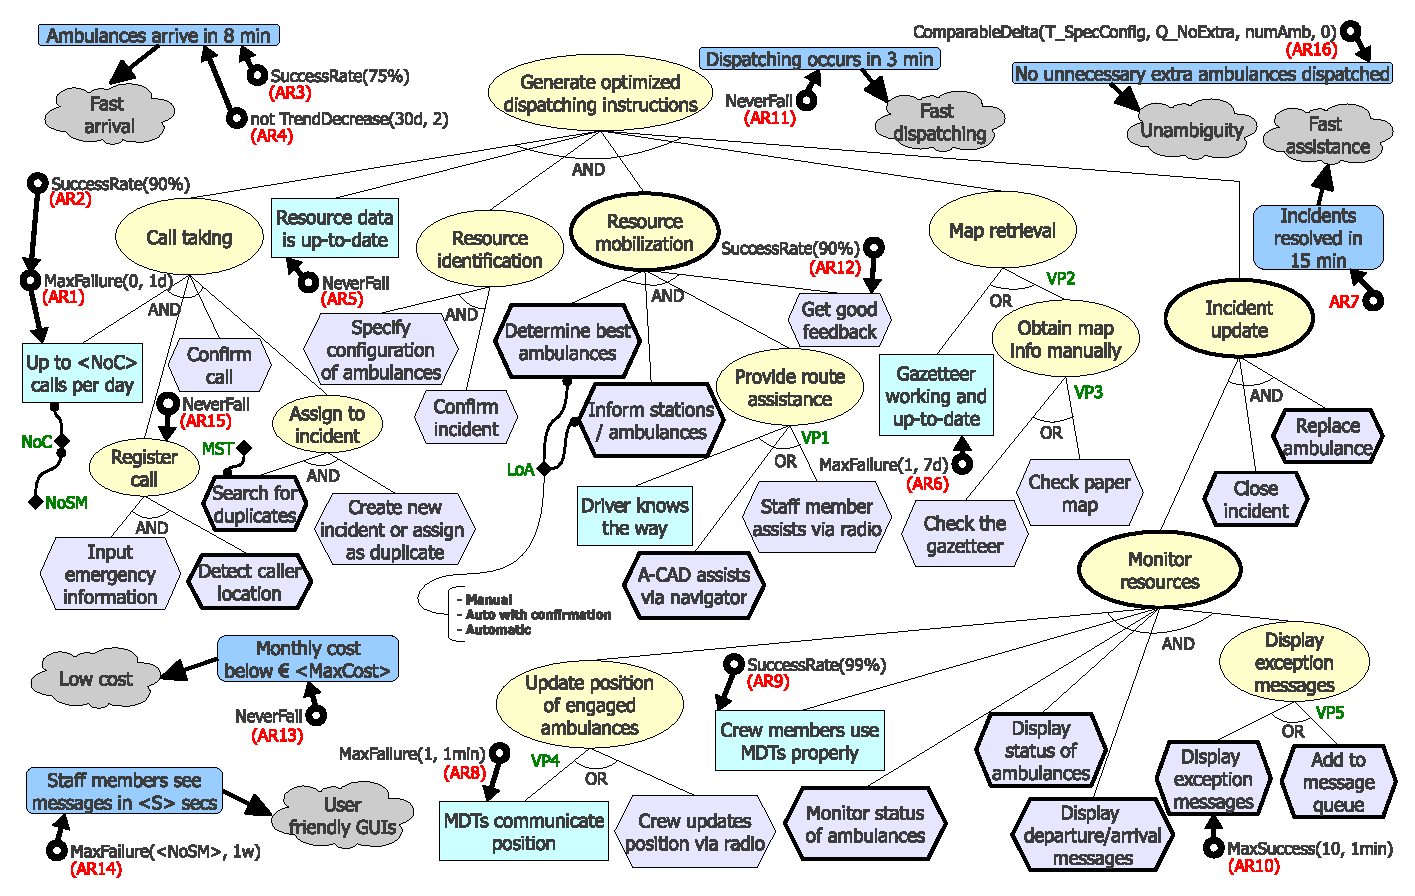
\includegraphics[width=\textwidth]{figuras/fig-intro-exemplosideways} 
\caption{Exemplo de figura em modo paisagem: um modelo de objetivos~\cite{souza-mylopoulos:spe13}.}
\label{fig-intro-exemplosideways}
\end{sidewaysfigure}



%%% Início de seção. %%%
\section{Tabelas}
\label{sec-intro-tabelas}

Tabelas são um ponto fraco do \latex. Elas são complicadas de fazer e, dependendo da complexidade da tabela (muitas células mescladas, por exemplo), vale a pena construi-las em outro programa (por exemplo, em seu editor de texto favorito), converter para PDF e inclui-las no documento como figuras. Mostramos, no entanto, alguns exemplos de tabela a seguir. O código utilizado para criar as tabelas encontra-se nas listagens~\ref{lst-intro-tabelas01} e~\ref{lst-intro-tabelas02}. 

\lstinputlisting[label=lst-intro-tabelas01, caption=Código \latex utilizado para inclusão das tabelas~\ref{tbl-intro-exemplo01} e~\ref{tbl-intro-exemplo02}., float=htpb]{codigos/lst-intro-tabelas01.tex}

\lstinputlisting[label=lst-intro-tabelas02, caption=Código \latex utilizado para inclusão da Tabela~\ref{tbl-intro-exemplo03}., float=htpb]{codigos/lst-intro-tabelas02.tex}

% Exemplo de tabela 01:
\begin{table}
\caption{Exemplo de tabela com diferentes alinhamentos de conteúdo.}
\label{tbl-intro-exemplo01}
\centering
\begin{tabular}{ | c | l | r | p{40mm} |}\hline
\textbf{Centralizado} & \textbf{Esquerda} & \textbf{Direita} & \textbf{Parágrafo}\\\hline
C & L & R & Alinhamento de tipo parágrafo especifica largura da coluna e quebra o texto automaticamente.\\
\hline
Linha 2 & Linha 2 & Linha 2 & Linha 2\\
\hline
\end{tabular}
\end{table}

% Exemplo de tabela 02:
\begin{table}
\caption{Exemplo que especifica largura de coluna e usa lista enumerada (adaptada de~\cite{souza-mylopoulos:spe13}).}
\label{tbl-intro-exemplo02}
\centering
\renewcommand{\arraystretch}{1.2}
\begin{small}
\begin{tabular}{ | p{15mm} | p{77mm} | p{55mm} |}\hline
\textbf{\textit{AwReq}} & \textbf{Adaptation strategies} & \textbf{Applicability conditions}\\\hline

AR1 &
\vspace{-2mm}\begin{enumerate}[topsep=0cm, partopsep=0cm, itemsep=0cm, parsep=0cm, leftmargin=0.5cm]
\item \textit{Warning(``AS Management'')}
\item \textit{Reconfigure($\varnothing$)}
\end{enumerate}\vspace{-4mm} &
\vspace{-2mm}\begin{enumerate}[topsep=0cm, partopsep=0cm, itemsep=0cm, parsep=0cm, leftmargin=0.5cm]
\item Once per adaptation session;
\item Always.
\end{enumerate}\vspace{-4mm}
\\\hline

AR2 &
\vspace{-2mm}\begin{enumerate}[topsep=0cm, partopsep=0cm, itemsep=0cm, parsep=0cm, leftmargin=0.5cm]
\item \textit{Warning(``AS Management'')}
\item \textit{Reconfigure($\varnothing$)}
\end{enumerate}\vspace{-4mm} &
\vspace{-2mm}\begin{enumerate}[topsep=0cm, partopsep=0cm, itemsep=0cm, parsep=0cm, leftmargin=0.5cm]
\item Once per adaptation session;
\item Always.
\end{enumerate}\vspace{-4mm}
\\\hline
\end{tabular}
\end{small}
\end{table}

% Exemplo de tabela 03:
\begin{table}
\caption{Exemplo que mostra equações em duas colunas (adaptada de~\cite{souza-mylopoulos:spe13}).}
\label{tbl-intro-exemplo03}
\centering
\vspace{1mm}
\fbox{\begin{minipage}{.98\linewidth}
\begin{minipage}{0.51\linewidth}
\vspace{-4mm}
\begin{eqnarray}
\Delta \left( I_{AR1} / NoSM \right) \left[ 0, maxSM \right] > 0\\
\Delta \left( I_{AR2} / NoSM \right) \left[ 0, maxSM \right] > 0\\
\Delta \left( I_{AR3} / LoA \right) < 0\\
\end{eqnarray}
\vspace{-6mm}
\end{minipage}
\hspace{2mm}
\vline 
\begin{minipage}{0.41\linewidth}
\vspace{-4mm}
\begin{eqnarray}
\Delta \left( I_{AR11} / VP2 \right) < 0\\
\Delta \left( I_{AR12} / VP2 \right) > 0\\
\Delta \left( I_{AR6} / VP3 \right) > 0\\
\end{eqnarray}
\vspace{-6mm}
\end{minipage}
\end{minipage}}
\end{table}
% ==============================================================================
% TCC - Nome do Aluno
% Capítulo 2 - Referencial Teórico
% ==============================================================================
\chapter{Algoritmo de Dijkstra}
\label{sec-dijkstra}

\section{O Algoritmo}
\label{sec-dijkstra-algoritmo}
O algoritmo de Dijkstra foi proposto por Edgar W. Dijkstra em 1959 \cite{dijkstra1959note}. Ele tem por objetivo definir o menor caminho partindo do vértice origem $v_{s}$ e chegando a todos os demais vértices $v_{i}$ do grafo $G = (V,E)$. Para garantir a viabilidade do algoritmo, assume-se que todos os pesos $w( u, v )$ sejam maiores ou iguais a zero para toda aresta $E$ do grafo $G$ \cite{cormen2009introduction}.

A seguir é apresentado o pseudocódigo do algoritmo conforme descrito em \citeonline{drozdek2012data}.
%\begin{verbatim}
%CÓDIGO AQUI
%\end{verbatim}

\begin{lstlisting}[ mathescape, label=lst-dijkstra-codigo, caption=Algoritmo de Dijkstra., float=htpb]
DijkstraAlgorithm(weighted simple digraph, vertex first)
	for all vertices v
		currDist(v) = $\infty$;
	currDist(first) = 0;
	toBeChecked = all vertices;
	while toBeChecked is not empty
		v = a vertex in toBeChecked with minimal currDist(v);
		remove v from toBeChecked;
		for all vertices u adjacent to v and in toBeChecked
			if currDist( u ) > currDist( v ) + weight( edge(vu) )
				currDist( u ) = currDist( v ) + weight( edge(vu) );
				predecessor( u ) = v;
\end{lstlisting}

%\begin{verbatim}
%DijkstraAlgorithm(weighted simple digraph, vertex first)
%	for all vertices v
%	currDist(v) = infinite;
%	currDist(first) = 0;
%	toBeChecked = all vertices;
%	while toBeChecked is not empty
%		v = a vertex in toBeChecked with minimal currDist(v);
%		remove v from toBeChecked;
%		for all vertices u adjacent to v and in toBeChecked
%		if currDist( u ) > currDist( v ) + weight( edge(vu) )
%			currDist( u ) = currDist( v ) + weight( edge(vu) );
%			predecessor( u ) = v;
%\end{verbatim}

O algoritmo inicia atribuindo o valor inicial de cada distância de cada vértice do grafo igual a $\infty$, com exceção do vértice inicial $v_{s}$ que será iniciado por 0. Em seguida todos os vértices são adicionados ao conjunto dos "toBeChecked" ("aSeremChecados"). Feito isso, inicia-se o processo iterativo: seleciona-se o vértice $v$ de menor custo que esteja dentro do conjunto "toBeChecked", retira-se ele do conjunto e a partir dele, para cada vértice adjacente $u$ de $v$, verifica-se se a distância atual calculada de $u$ é maior do que a distância calculada de $v$ mais o valor referente ao peso da aresta de $v$ e $u$ (origem em $v$). Caso seja verdade, a distância atual de $u$ é substituída pela soma da distância atual de $v$ mais o peso da aresta de $v$ e $u$ (este valor corresponde à distância do vértice de origem $v_{s}$ até $u$), além de definir o antecessor $u$ como $v$. Repete-se o passo iterativo até que o conjunto "toBeChecked" esteja vazio\footnote{Em linguagens de programação, é costume substituir o valor $\infty$ pelo maior número representativo do tipo da variável selecionado para representar a distância. Por exemplo na linguagem C, caso se utilize o valor int (inteiro) para representar a distância, a atribuição inicial será dado pela constante INT\underline{\space}MAX  definida pela biblioteca "limits.h", que representa o maior valor numérico representado por esse tipo de variável.}.
\newpage
Ao final do algoritmo, teremos o conjunto de predecessores de cada vértice do grafo, e a partir deste, poderemos definir a rota para qualquer vértice do grafo partindo de $v_{s}$. O caminho retornado é garantidamente ótimo como mostra \citeonline{cormen2009introduction}.

A figura \ref{fig-dijkstra-algoritmo-grafo} mostra um exemplo de aplicação do algoritmo a um grafo.

\begin{figure}[H]
\centering
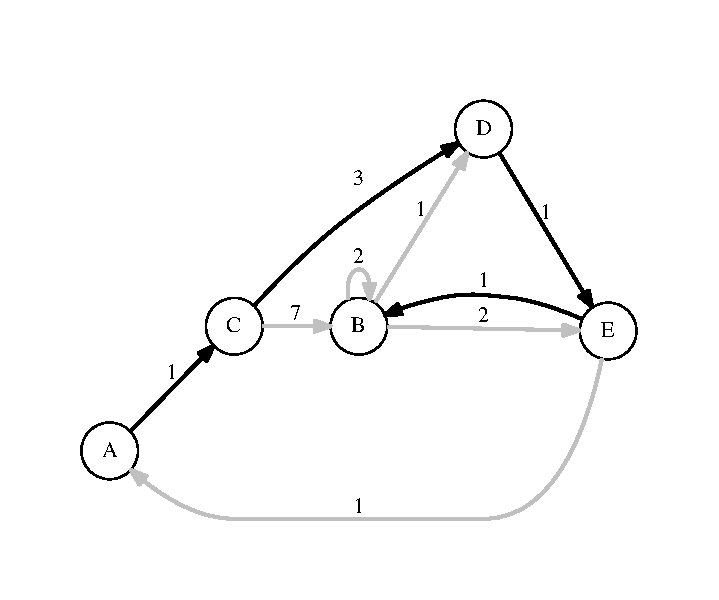
\includegraphics[width=1.\textwidth]{figuras/grafo-dijkstra} 
\caption{Aplicação do algoritmo de Dijkstra tendo o vértice "A" como origem. As arestas pintadas de preto correspondem a rota calculada a todos os demais vértices.}
\label{fig-dijkstra-algoritmo-grafo}
\end{figure}

Inicialmente a distância do vértice "A" é atribuído como zero enquanto de todos os demais é atribuído como infinito $\infty$. Inicia-se o processo iterativo a partir de "A" que explora os seus vértices adjacentes, que neste caso só tem um que é o vértice "C". A distância de "C" é calculada como o valor da distância de "A" mais o peso da aresta "AC" (que é igual a 1), e o vértice que é atribuído como antecessor de "C" é "A". Em seguida é escolhido o vértice cuja a distância seja a menor dentro do conjunto "toBeChecked" que neste caso é o próprio "C". Do vértice "C" explora-se os vértices adjacentes dele "D" e "B". Suas respectivas distâncias são atribuídas como a distância de "C" mais o peso de suas respectivas arestas (currDist( B ) = 7 + 1; currDist( D ) = 3 + 1), além de atribuir como "C" os seus respectivos vértices antecessores. Disso novamente, escolhe-se o vértice com menor distância em "toBeChecked" que neste caso será o D (currDist( D ) = 4 < currDist( C ) = 8). De "D" é explorado seu vértice adjacente "E" que é atribuído seu valor currDist( E ) como sendo 5 (3 + 1 + 1) e seu vértice antecessor como "D". Busca-se novamente o menor valor dos vértices em "toBeChecked" que neste caso será o "E" (currDist( E ) = 5 < currDist( B ) = 8). Dele explora-se os seus vértices adjacentes "B" e "A". O único valor da distância que é alterado é o de "B" pois o caminho vindo por "E" (A->C->D->E = 1 + 3 + 1 + 1) é menor do que o vindo por "C"  (A->C->B = 1 + 7). Finalmente, o vértice "B" é explorado, mas nenhum de seus vértices adjacentes tem o valor de sua distância alterado pois o menor caminho para eles já foi encontrado.

\section{Versões do Algoritmo implementadas e suas Estrutura de Dados}
\label{sec-dijkstra-versoes}
Para este projeto de graduação será implementada três versões do algoritmo de Dijkstra baseados em estruturas de dados diversas que implicam em tempos computacionais diferentes \cite{cormen2009introduction}.

As versões implementadas são o Dijkstra Canônico (descrito a seguir), Dijkstra Heap Binário (subseção \ref{sec-dijkstra-versoes-heap}) e Dijkstra Heap de Fibonacci (subseção \ref{sec-dijkstra-versoes-fibonacci}), todas baseadas em \citeonline{cormen2009introduction, drozdek2012data}.

Para a versão Dijkstra Canônico o algoritmo utiliza de um vetor para armazenar as distâncias calculadas pelo algoritmo (o indíce dos vértices correspondem ao indíce do vetor em que são armazenados), e a cada passo iterativo (conforme demonstrado pelo algoritmo na seção \ref{sec-dijkstra-algoritmo}), uma busca linear é realizada para determinar o vértice (fora do conjunto "toBeChecked") cuja a distância é menor dentre todas as outras. O tempo computacional para esse caso é $O(|V^{2}|)$ \cite{drozdek2012data}.

\subsection{Dijkstra Heap Binário}
\label{sec-dijkstra-versoes-heap}
Para esta implementação, será utilizada a estrutura de dados heap binária mínima como fila de prioridade. Heaps binária podem ser descritas como árvores binárias que possuem as seguintes propriedades \cite{drozdek2012data}:
\begin{enumerate}
 \item O valor de cada nodo não é maior do que os valores guardados em cada um de seus filhos.
 \item A árvore é perfeitamente balanceada, e as folhas no último nível estão todas mais a esquerda.
\end{enumerate}

Um exemplo de estrutura Heap Binário representada tanto como árvore como vetor pode ser visualizado nas figuras \ref{fig-dijkstra-heapbinario} e \ref{fig-dijkstra-heapvetor} respectivamente.

\begin{figure}[H]
\centering
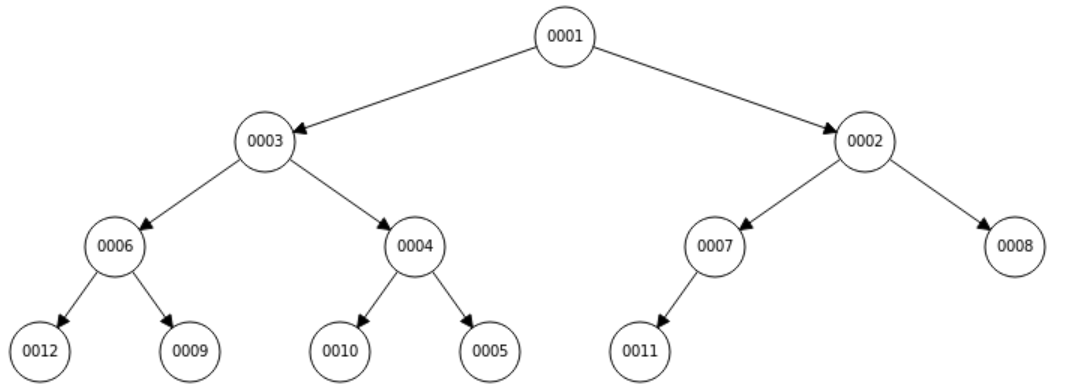
\includegraphics[width=.95\textwidth]{figuras/Heap} 
\caption{Exemplo de Heap Binário representado como árvore.}
\label{fig-dijkstra-heapbinario}
\end{figure}

\begin{figure}[H]
\centering
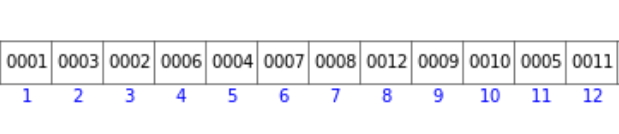
\includegraphics[width=.60\textwidth]{figuras/Heap-vetor}
\caption{Representação do Heap Binário da figura \ref{fig-dijkstra-heapbinario} como vetor.}
\label{fig-dijkstra-heapvetor}
\end{figure}

A disposição dos elementos da árvore no vetor segue as seguintes relações entre nós pai, filho-direita e filho-esquerda:
%\begin{equation}
%Pai(i): \lfloor i/2 \rfloor
%\end{equation}
%\begin{equation}
%Filho-esquerda(i): 2*i
%\end{equation}
%\begin{equation}
%Filho-direita(i): 2*i+1
%\end{equation}
\begin{description}
\item[Pai($i$):] $\lfloor i/2 \rfloor$
\item[Filho-esquerda($i$):] $2*i$
\item[Filho-direita($i$):] $2*i+1$
\end{description}
Onde $i \in \mathbb{N}$ e $i \subset [1, n]$, sendo que $i$ representa o índice do elemento no vetor e $n$ o número de elementos da árvore.

 Para efeito de exemplo (observe as figuras \ref{fig-dijkstra-heapbinario} e \ref{fig-dijkstra-heapvetor} para constatação), o nó que está contido na posição 4 do vetor possui como pai o nó de posição 2 ($\lfloor 4 / 2 \rfloor = 2$), tem como filho da esquerda o nó de posição 8 ($2*4 = 8$) e filho da direita o nó de posição 9 ($2*4+1 = 9$).

%\begin{equation}
%\forall i, i \in \mathbb{N} [1,n]
%\end{equation}

A vantagem de se usar essa estrutura de dados reside no fato de suas operações de inserção, extração de mínimo e reconstrução da heap possuirem tempo computacional de $O(\lg n)$. Por consequência, o tempo computacional para este caso é de $O(|E| \lg |V|)$ \cite{cormen2009introduction}.

\subsection{Dijkstra Heap de Fibonacci}
\label{sec-dijkstra-versoes-fibonacci}
A Heap de Fibonacci consiste de uma coleção de árvores que seguem a regra de árvore heap mínima, ou seja, os nós pais são maiores ou iguais aos nós filhos. Os nós raízes de cada árvore são interligados por uma lista circular duplamente encadeada. Um ponteiro chamado "raiz mínima" aponta para o nó de menor valor.

Sua característica é que operações de adição são executadas de uma maneira "preguiçosa", não procurando criar uma forma para as árvores (como por exemplo, deixa-la balanceada), apenas as adicionados-as a lista principal de raízes. Por consequência, operações de inserção possuem tempo computacional $O(1)$ \cite{cormen2009introduction}.

\begin{figure}[H]
\centering
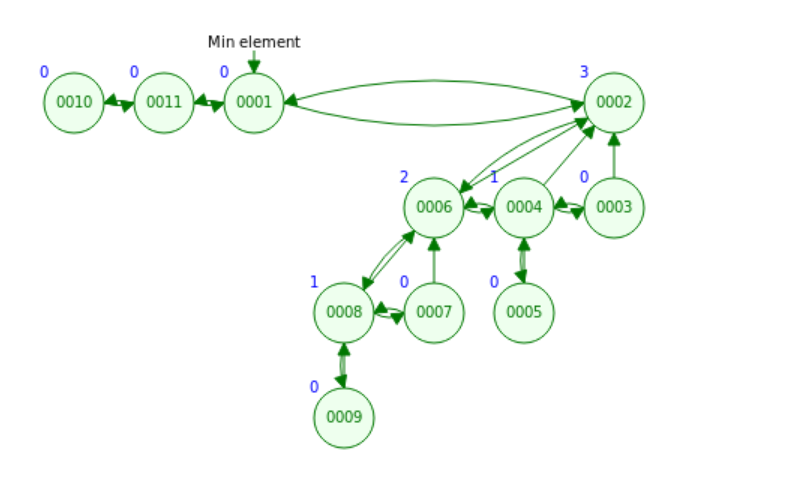
\includegraphics[width=.54\textwidth]{figuras/fibonacci-heap1} 
\caption{Exemplo de Heap de Fibonacci (os números no canto superior esquerdo de cada nodo correspondem ao grau de cada um, ou seja, o número de filhos).}
\label{fig-dijkstra-heapfibonacci1}
\end{figure}

Para operações de extração de mínimo o tempo computacional é mais custoso. Isso é devido ao fato de que quando o mínimo é retirado, a heap precisa ser reorganizada de forma que sua propriedade principal não seja violada e o um novo mínimo seja determinado. Para isso a operação de extração de mínimo se dá em três etapas. Primeiro é retirado o mínimo da heap (se caso o mínimo possua nós filhos, eles são colocados na lista principal de raízes) e o seu vizinho é assimilado como o novo mínimo provisório. Agora precisamos definir quem é o novo mínimo e para isso teremos que verificar todos os demais nós raízes. Com o intuito de diminuir o número de nós raízes é que o segundo passo é aplicado.  Ele consiste em lincar raízes com o mesmo número de grau (grau corresponde ao número de filhos que cada nodo possui) e para cada par de nodos licandos, verifica-se qual dos dois é menor. O que for o menor será o nodo pai e outro por consequência será o nodo filho. Após a lincagem de todos os nodos com mesmo número de grau, uma busca linear é realizada para se determinar o menor elemento entre os nodos raízes restantes\footnote{Para otimizar a busca de nodos com o mesmo número de grau é utilizado um vetor auxiliar de tamanho mínimo ao maior grau de um nodo da estrutura. Esse vetor contém ponteiros para os nodos e a posição desse nodo no ponteiro corresponde ao grau do nodo. Por exemplo, se um nodo possui grau 3, ele ocupará a posição de número 3 no vetor. Quando um nodo da lista é referenciado na posição que já está ocupado, o processo de lincagem é feito conforme descrito.}. O tempo computacional para a extração de mínimo é $O(\lg n)$ \cite{cormen2009introduction}.

%\footnote{Para otimizar a busca de nodos com o mesmo número de grau é utilizado um vetor auxiliar de tamanho mínimo ao maior grau de um nodo da estrutura. Esse vetor contém ponteiros para os nodos e a posição desse nodo no ponteiro corresponde ao grau do nodo. Por exemplo, se um nodo possui grau 3, ele ocupará a posição de número 3 no vetor. Quando um nodo da lista é referenciado na posição que já está ocupado, o processo de lincagem é feito conforme descrito.}

\begin{figure}[H]
\centering
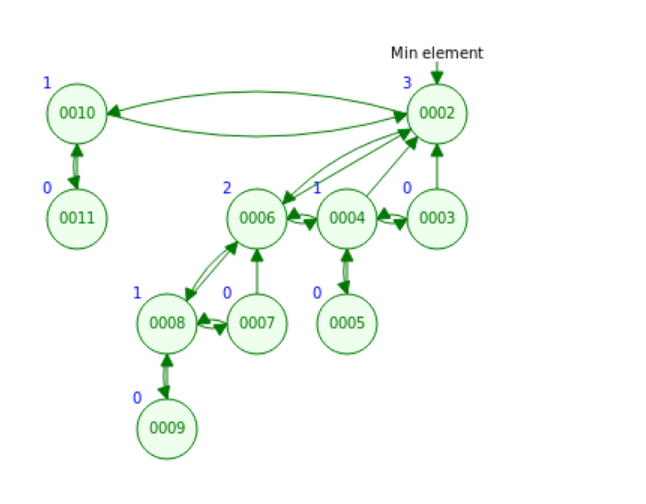
\includegraphics[width=.54\textwidth]{figuras/fibonacci-heap2} 
\caption{Heap de Fibonacci da figura \ref{fig-dijkstra-heapfibonacci1} após a operação de extração de mínimo.}
\label{fig-dijkstra-heapfibonacci2}
\end{figure}


Finalmente para a operação de mudança de chave de um determinado nodo, e após a mudança realizada em tempo constante ($O(1)$), é verificado se a propriedade heap foi violada. Se caso sim, esse nodo é cortado de seu nodo pai e colocado junto a lista principal. Se o pai não pertencer a lista de nodos raízes, ele é "marcado" ("pintado") e caso já estivesse "marcado" ele também é cortado e seu pai é "marcado". Esse processo continua subindo até encontrarmos um nodo pai "não marcado" ou um nodo raiz. Após esse processo recursivo ter terminado, verifica-se se nodo modificado inicialmente é menor do que o nodo mínimo atual. Se caso sim, o novo nodo mínimo é o modificado. O tempo computacional é $O(1)$ \cite{cormen2009introduction}.

Por consequência, o tempo computacional aplicado para o algoritmo de Dijkstra é de $O(|V|\lg |V| + |E|)$ \cite{cormen2009introduction}.
% ==============================================================================
% TCC - Nome do Aluno
% Capítulo 3 - Especificação de Requisitos
% ==============================================================================
\chapter{Algoritmo A*}
\label{sec-aestrela}

\section{O Algoritmo}
\label{sec-aestrela-algoritmo}
O algoritmo A* (lê-se "A estrela") também conhecido como busca A* é um algoritmo de busca informatizada em grafos. Foi proposta originalmente em (buscar referência) e pode ser visto como uma adaptação do algoritmo de Dijkstra (apresentado no capítulo \ref{sec-dijkstra}) em que, ao invés de se calcular a melhor rota de um ponto de partida para todos os demais vértices do grafo, se estabelece uma boa rota (ou mesmo a rota ótima\footnote{A garantia do valor ótimo do algoritmo depende de fatores que serão discutidos na subseção \ref{sec-aestrela-algoritmo-heuristica}.}) partindo do vértice origem a um vértice destino. Isso é feito realizando "podas" do caminho de forma que não seja necessário visitar todos os vértices, apenas os mais promissores.

A seguir é apresentado o algoritmo A* adaptado de \citeonline{likhachev2008anytime} sobre o algoritmo de Dijkstra apresentado na seção \ref{sec-dijkstra-algoritmo}. 

\begin{lstlisting}[ mathescape, label=lst-aestrela-codigo, caption=Algoritmo A*, float=htpb]
$A^{*}$Algorithm(weighted simple digraph, vertex first, vertex goal)
	for all vertices v
		g(v) = $\infty$;
	g(first) = 0;
	toBeChecked = all vertices;
	while goal is in toBeChecked
		v = a vertex in toBeChecked with minimal f(v);
		remove v from toBeChecked;
		for all vertices u adjacent to v and in toBeChecked
			if g( u ) > g( v ) + weight( edge(vu) )
				g( u ) = g( v ) + weight( edge(vu) );
				predecessor( u ) = v;
				update u in toBeChecked with f(u) = g(u) + h(u);
\end{lstlisting}

O algoritmo segue em sua essência como um Dijkstra adaptado. Iniciamos a distância de todos os vértices g(v) como sendo $\infty$\footnote{Vide nota de rodapé da seção \ref{sec-dijkstra-algoritmo}.} (o valor de g(v) corresponde ao valor da distância calculada do vértice origem "first" até o vértice "v") com exceção do vértice origem, cujo valor atribuído é zero. Adicionamos todos os vértices ao grupo dos "toBeChecked" \footnote{Algumas literaturas designam esse conjunto como OPEN.}. Feito isso inicia-se o processo iterativo: enquanto o vértice "goal" estiver dentro do conjunto do "toBeChecked" (ou seja, o vértice "goal" não foi alcançado ainda pelo algoritmo), o vértice com menor valor f(v) é retirado do conjunto "toBeChecked" e para cada vértice adjacente u de v, verifica-se se o valor de g( u ) atual é maior que g( v ) mais o peso da aresta entre v e u (edge(vu)). Se caso for verdade, o valor de g( u ) é atualizado para g( v ) mais o peso da aresta entre v e u, e v é marcado como o predecessor de u. O valor do peso do vértice u é atualizado na fila de prioridades utilizada (como a heap binária, descrita na subseção \ref{sec-dijkstra-versoes-heap}) com o valor f( u ) = g( u ) + h( u ).

Observe que para o algoritmo A*, diferente do que ocorre em Dijkstra, não utiliza o valor de g( u ) (valor da distância calculada do vértice origem "first" até o vértice "u") como chave de ordenamento da fila de prioridade, mas sim esse valor acrescido de h( u ). Observe também que o algoritmo para ao ser removido o vértice destino ("goal") da lista do "toBeChecked" em contrapartida ao Dijkstra que calcula para todos os vértices do grafo.

O termo h( u ) significa o valor heurístico que corresponde a uma estimativa da distância de u ao vértice destino "goal". É devido a esse valor que o algoritmo A* realiza "podas" no número de vértices a serem checados, buscando os mais promissores, já que o valor heurístico faz com que os vértices cujas estimativas sejam mais próximas do vértice destino ("goal") sejam colocados mais a frente na fila de prioridades e por consequência, sejam calculadas primeiros. E assim é mais provável que o vértice destino seja alcançado antes e tenha sua rota calculada, terminando o algoritmo. O valor h( u ) é classificado como admissível e não-admissível cujo significado será dado na subseção \ref{sec-aestrela-algoritmo-heuristica}.

A figura \ref{fig-aestrela-algoritmo-mapa1} contida em \citeonline{russell1995modern} mostra um exemplo de aplicação do algoritmo [DESCREVER A FIGURA AQUI].

\begin{figure}[H]
\centering
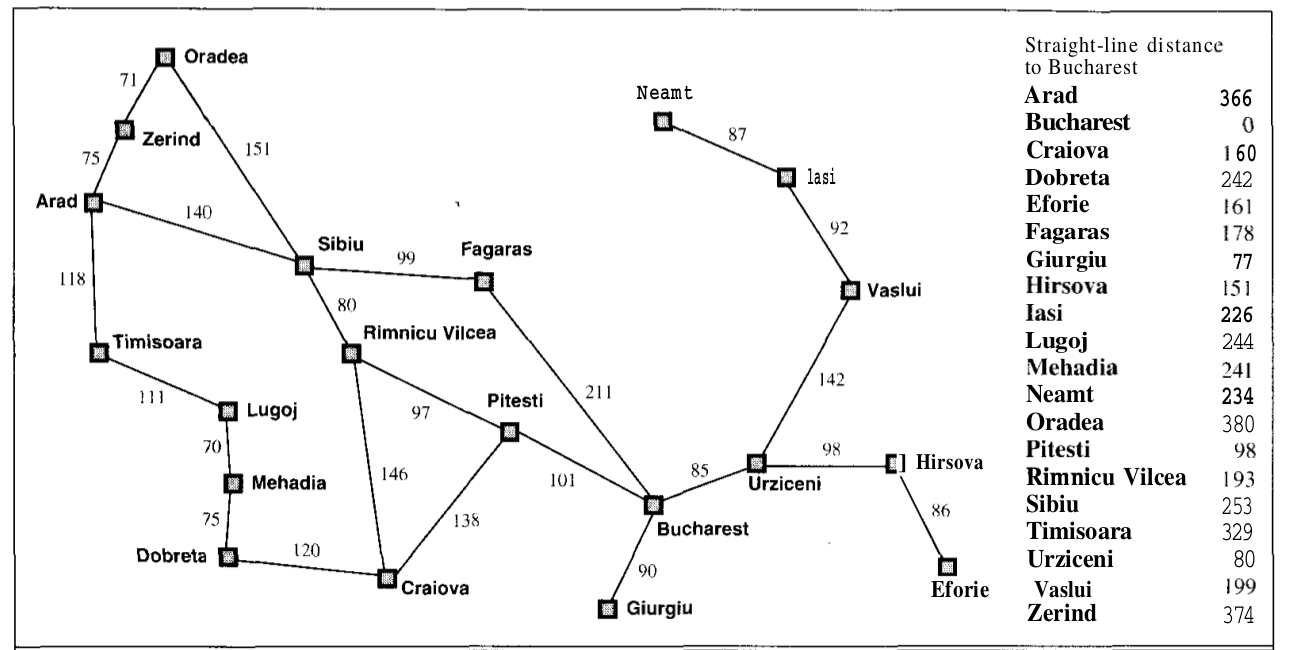
\includegraphics[width=.90\textwidth]{figuras/Aestrela-mapa1} 
\caption{Mapa da Romênia com os valores das distâncias entre as cidades, e a distância euclidiana até Bucareste.}
\label{fig-aestrela-algoritmo-mapa1}
\end{figure}

\begin{figure}[H]
\centering
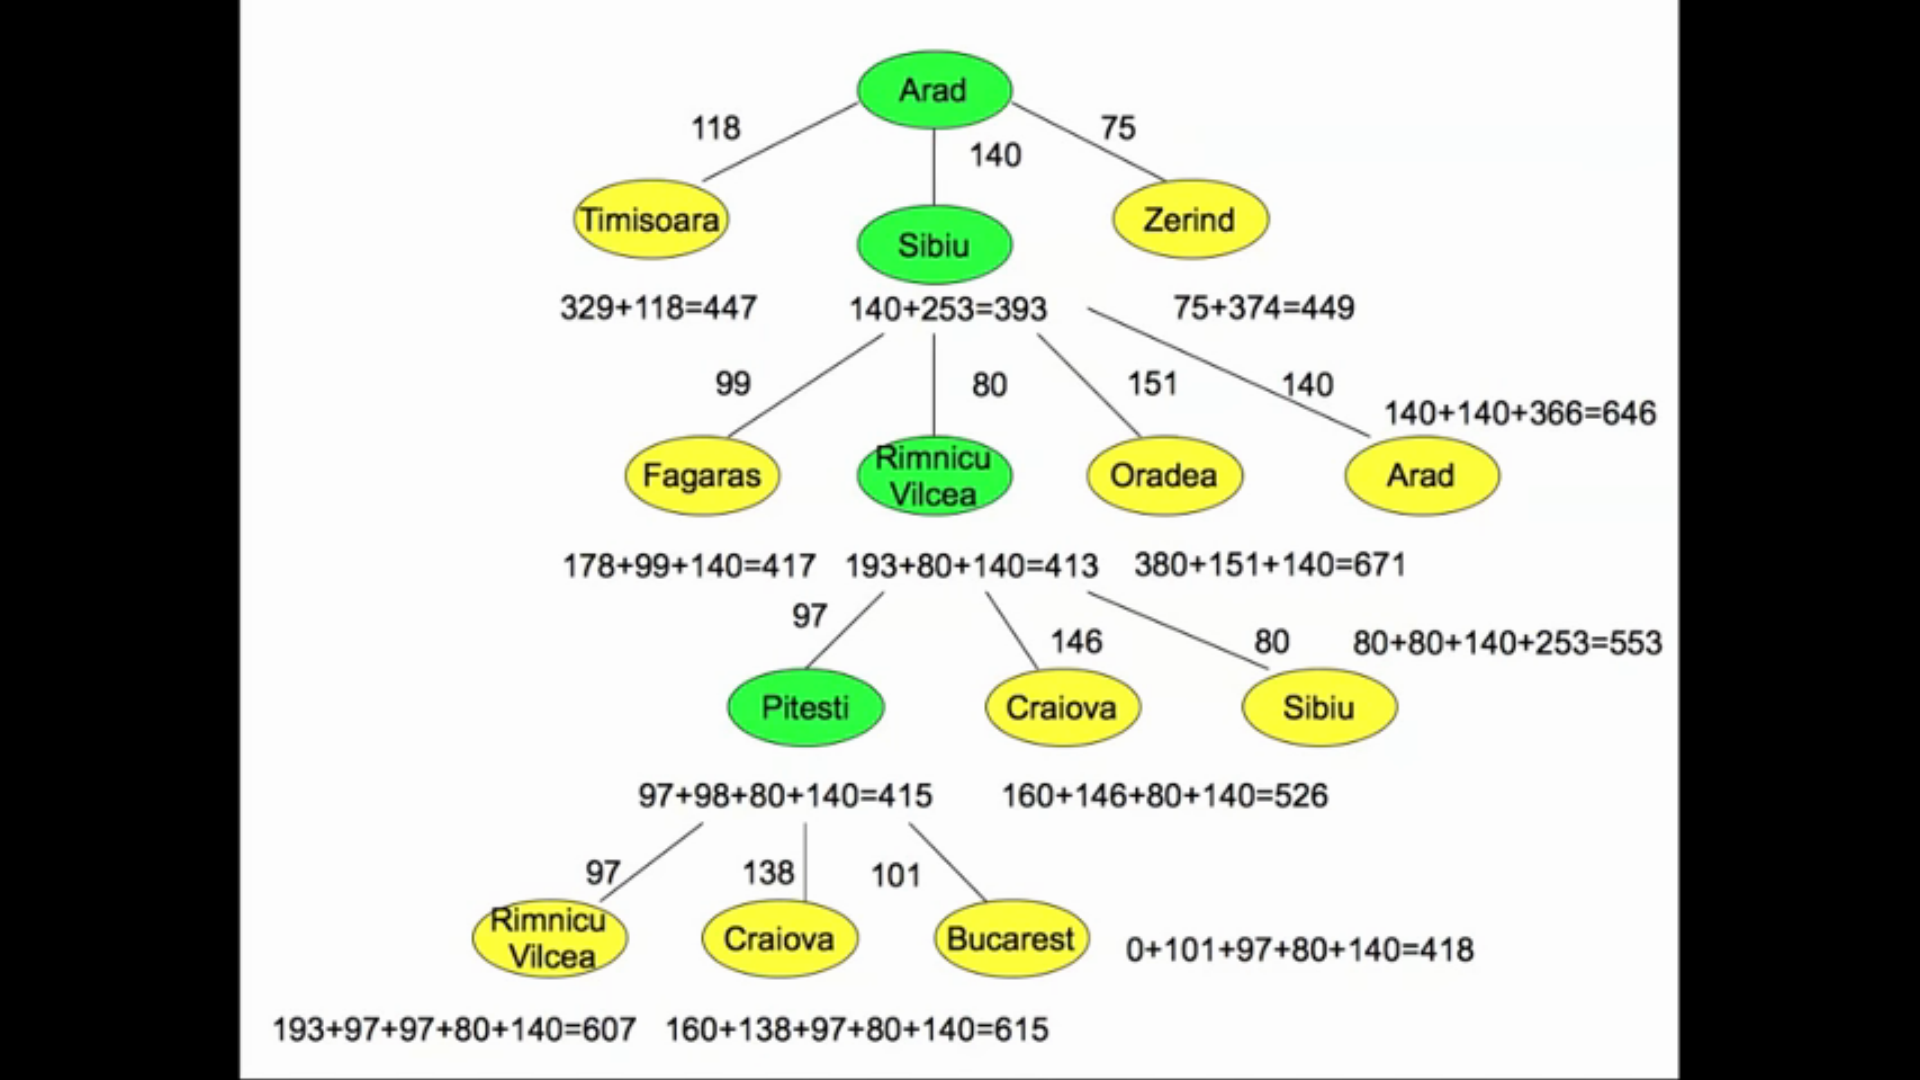
\includegraphics[width=.90\textwidth]{figuras/Aestrela-mapa2} 
\caption{Desenvolvimento do algoritmo A* (MUDAR DEPOIS)}
\label{fig-aestrela-algoritmo-mapa2}
\end{figure}


%\citeonline{russell1995modern,cormen2009introduction}.

%\begin{lstlisting}[ mathescape, label=lst-aestrela-codigo, caption=Algoritmo A*, float=htpb]
%Entrada: Grafo G, vértice inicial $v_{i}$, vértice destino $v_{f}$
%	para todo vértice $s \in V(G), s \neq vi$ faça
%		$g(s) = \infty$
%	fim para
%	$g(v_{i}) = 0$
%	para todo vértice $s \in V(G)$ faça
%		anterior($s$) = -1
%	fimpara
%	OPEN = {$v_{i}$}
%	enquanto $v_{f}$ não é expandido faça
%		s = desenfila(OPEN)
%		para cada sucessor $s'$ de $s$ faça
%			se $g(s') > g(s) + c(s,s')$ então
%				$g(s') = g(s) + c(s,s')$
%				anterior($s'$) = s
%				insira/atualize $s'$ em OPEN pelo valor de f
%			fim se
%		fim para
%	fim enquanto
%retorna anterior
%\end{lstlisting}



\subsection{Heurísticas admissíveis e não-admissíveis}
\label{sec-aestrela-algoritmo-heuristica}  

\section{Experimentos Computacionais}
\label{sec-aestrela-experimentos}

% ==============================================================================
% TCC - Nome do Aluno
% Capítulo 3 - Projeto Arquitetural e Implementação
% ==============================================================================
\chapter{Algoritmos Dinâmicos}
\label{sec-dinamicos}

\section{Grafos Dinâmicos}
\label{sec-dinamicos-grafos}
Os algoritmos apresentados até agora tratam apenas de grafos estáticos, ou seja, grafos em que o peso de suas arestas não mudam. Mas em situações reais podemos ter casos em que a modelagem feita por grafos requer que os pesos de suas arestas variem com o tempo. Para esses casos, temos grafos ditos \textbf{dinâmicos}. Exemplos de modelagem por grafos dinâmicos são o sistema de tempo real de trânsito em que os pesos das arestas correspondem ao tempo médio para percorrer um determinado trecho e esse tempo está diretamente ligado ao trânsito local em uma determinada hora; e o fluxo de em uma rede interna onde as arestas representam o caminho entre roteadores e os seus pesos correspondem ao uso desta linha, ou seja, o quão congestionada está.

Para calcularmos o menor caminho entre dois vértices em grafos dinâmicos, poderíamos utilizar os algoritmos de Dijsktra e A* (discutidos nos capítulos \ref{sec-dijkstra} e \ref{sec-aestrela})  para acharmos a rota, e quando houver uma detecção de mudança do peso de arestas, recalcularíamos novamente o trajeto reutilizando esses algoritmos. Em geral desejamos (ou necessitamos) que esse recálculo seja mais rápido. Para esse fim existem os algoritmos dinâmicos que calculam uma solução rápida porém não garantidamente ótima (elas são ditas sub-ótimas).

Exemplos de algoritmos são o D* \cite{stentz1994optimal}, D* Lite \cite{koenig2002d} e o AD* \cite{likhachev2008anytime}.

Será discutidos os algoritmos ARA* e AD* \cite{likhachev2008anytime}, que foram escolhidos para serem estudados por este trabalho.
\section{Algoritmo ARA*}
\label{sec-dinamicos-ara}

O algoritmo ARA* proposto em \citeonline{likhachev2008anytime}, está descrito nos algoritmos \ref{lst-dinamicos-ara-computepath}, \ref{lst-dinamicos-ara-key} e \ref{lst-dinamicos-ara-main}.

\begin{lstlisting}[mathescape, label=lst-dinamicos-ara-computepath, caption=Algoritmo ARA* - função de cálculo de caminho, float=htpb]
procedure ComputePath()
	while(key($s_{goal}$) > $min_{s \in OPEN(key(s))}$)
		remove s with smallest key(s) from OPEN;
		v(s) = g(s); CLOSED = CLOSED $\cup$ {s};
		for each successor s' of s
			if s' was never visited by ARA* before then
				v(s') = g(s') = $\infty$;
			if g(s') > g(s) + c(s, s')
				g(s') = g(s) + c(s, s');
				if s' $\notin$ CLOSED
					insert/update s' in OPEN with key(s');
				else
					insert s' into INCONS;
\end{lstlisting}

 
\begin{lstlisting}[mathescape, label=lst-dinamicos-ara-key, caption=Algoritmo ARA* - função da chave ordenadora da fila de prioridades, float=htpb]
procedure key(s)
	return g(s) + $\epsilon$ * h(s);
\end{lstlisting}

\begin{lstlisting}[mathescape, label=lst-dinamicos-ara-main, caption=Algoritmo ARA* - função principal, float=htpb]
procedure Main()
	g($s_{goal}$) = v($s_{goal}$) = $\infty$; v($s_{start}$) = $\infty$;
	g($s_{start}$) = 0; OPEN = CLOSED = INCONS = $\emptyset$;
	insert $s_{start}$ into OPEN with key($s_{start}$);
	ComputePath();
	publish current $\epsilon$-suboptimal solution;
	while $\epsilon > 1$
		decrease $\epsilon$;
		Move states from INCONS into OPEN
		Update the priorities for all s $\in$ OPEN according to key(s);
		CLOSED = $\emptyset$;
		ComputePath();
		publish current $\epsilon$-suboptimal solution;
\end{lstlisting}

A função principal é descrita no Algoritmo \ref{lst-dinamicos-ara-main}. Temos as variáveis g(s) e v(s) que correspondem ao valor da distância real calculada da origem $s_{start}$ até o vértice s (o valor de v(s), apesar de estar descrito no algoritmo conforme a literatura de origem, não é utilizado pelo algoritmo. Ela é utilizada, na verdade, no próximo algoritmo, AD*, que está descrito no mesmo artigo do ARA* e foi do critério de seus autores originais colocar essa variável em sua descrição. Portanto será ignorado na explicação que se segue). O valor de g($s_{goal}$) (distância real calculada da origem ao vértice destino) é atribuído como $\infty$ (infinito)\footnote{Vide nota de rodapé da seção \ref{sec-dijkstra-algoritmo}.}, enquanto que o valor de g($s_{start}$) é atribuído com o valor 0 (já que o valor da distancia real é calculada a partir da origem). Em seguida são criados os conjuntos "OPEN", "CLOSED" e "INCONS", correspondendo respectivamente ao conjunto dos "ABERTOS", "FECHADOS" e "INCONSISTENTES". O vértice $s_{start}$ é inserido na fila de prioridades do conjunto OPEN utilizando a função de chave ordenadora descrito no algoritmo \ref{lst-dinamicos-ara-key}. Essa função utiliza a estratégia da heurística inflada (descrito a seguir, na subseção \ref{sec-dinamicos-ad-consideracoes}).

A função de cálculo de caminho é então acionada pela função principal (algoritmo \ref{lst-dinamicos-ara-computepath}). Nesta função, o processo iterativo se faz enquanto o valor da chave de $s_{goal}$ for maior do que o valor da chave do termo mínimo da fila de prioridades. Enquanto isso for verdade, o vértice s, que corresponde ao valor do vértice com menor chave de OPEN, é removido deste e adicionado ao conjunto CLOSED. Para cada s' (que representa um vértice do conjunto de vértices adjacentes de s) é verificado se o mesmo já foi visitado pelo algoritmo e em caso negativo, o seu valor de g(s') é atribuído como $\infty$ (infinito). Em seguida, é verificado se a distância calculada até o momento para s', g(s'), é maior do que a soma de g(s) com o peso da aresta entre s e s'. Se caso positivo, g(s') é atualizado com esse novo valor. Em seguida é verificado se o vértice s' não pertence ao conjunto dos fechados e em caso positivo, ele é adicionado/atualizado no conjunto OPEN de acordo com a função de chave ordenadora. Caso contrário, ele é adicionado ao conjunto dos INCONS.

Após o cálculo do caminho e de acordo com função principal (algoritmo \ref{lst-dinamicos-ara-main}), a solução $\epsilon$ sub-ótima (a explicação do motivo de a solução ser sub-ótima será dada na subseção \ref{sec-dinamicos-ara-consideracoes}) é apresentada pelo algoritmo. A partir daí começa o processo iterativo em que se verifica se o valor de $\epsilon$ é maior que 1. Em caso positivo, o valor de $\epsilon$ é decrescido por um fator de corte estipulado como parâmetro de entrada. Os vértices pertencentes a INCONS são movidos para OPEN e todas as chaves da fila de prioridades são atualizadas considerando o novo valor de $\epsilon$. O conjunto CLOSED é esvaziado e a função de cálculo de caminho é acionada novamente e seu respectivo resultado é apresentado.

\subsection{Heurística inflada e considerações sobre o algoritmo}
\label{sec-dinamicos-ara-consideracoes}

A principal diferença entre o algoritmo ARA* e o A* está na utilização da estratégia da heurística inflada. Ela consiste em utilizar a mesma função de ordenação de chaves da fila de prioridades do algoritmo A*, com a exceção de que o valor heurístico é multiplicado por um fator $\epsilon$. Isso faz com que menos vértices sejam visitados, já que os menos "promissores" serão posicionados mais para o final da fila de prioridades enquanto que os mais "promissores" serão posicionados mais para frente, e com isso é mais provável que um caminho até o vértice destino, $s_{goal}$, seja encontrado mais rápido do que pelo algoritmo A* (já que menos vértices deverão ser visitados). Entretanto, ao se utilizar esta técnica perdemos a garantia do resultado ótimo do algoritmo (algo semelhante ao que ocorre quando não utilizamos heurísticas não-admissíveis. Vide subseção \ref{sec-aestrela-algoritmo-heuristica}).

Porém, "Uma grande vantagem de se utilizar a estratégia apresentada é que temos um limite superior para a solução encontrada. Suponha que a melhor solução tenha custo C*. Se utilizarmos uma busca com o A* com um valor real $\epsilon \geq 1$ multiplicando o valor heurístico na função de avaliação, então há a garantia que para a nova solução C, C* $\leq$ C $\leq \epsilon$ x C*. Portanto, se $\epsilon$ = 1, a solução encontrada é ótima." \cite{moura2010estudo} \textbf{[A REVISAR]}.

Portanto a ideia principal é achar uma solução rápida, porém não-garantidamente ótima, atribuindo um valor $\epsilon$ maior do que 1, e caso a aplicação permita o uso de um tempo maior para aprimorarmos o resultado\footnote{Por exemplo, uma determinada aplicação necessita que se ache um caminho em no máximo 2 segundos. Se o algoritmo achar uma solução sub-ótima em 3 ms, dispomos de mais 1997 ms para podermos aprimorar ela.}, diminuímos o valor de $\epsilon$. E se o tempo ainda permitir, diminuímos até termos $\epsilon$ = 1, em que a solução será garantidamente ótima. 

Outra estratégia utilizada para ganhar tempo, a cada novo valor de $\epsilon$ em que a função para cálculo de caminho é acionada (algoritmo \ref{lst-dinamicos-ara-computepath}), não é necessário recalcular todos os vértices visitados anteriormente, já que os mesmos permanecem na lista de abertos (tendo apenas suas chaves atualizadas com o novo valor de $\epsilon$ e consequentemente a ordem dos vértices também é reconfigurada de acordo com esses novos valores). Além disso, caso haja um melhor caminho encontrado para um vértice que pertence aos fechados, este são colocados em INCONS \textbf{[PAREI AQUI]} dos quais serão enviados para OPEN para serem recalculados na próxima busca\footnote{Busca aqui, se refere ao número da iteração da invocação da função de cálculo de caminho (listagem \ref{lst-dinamicos-ara-computepath}), e consequentemente ao valor de $\epsilon$ a ele atribuído.}.

A figura \ref{fig-ara-exemplo}, contida em \citeonline{likhachev2008anytime}, mostra a aplicação da estratégia dita anteriormente.

\begin{figure}[H]
\centering
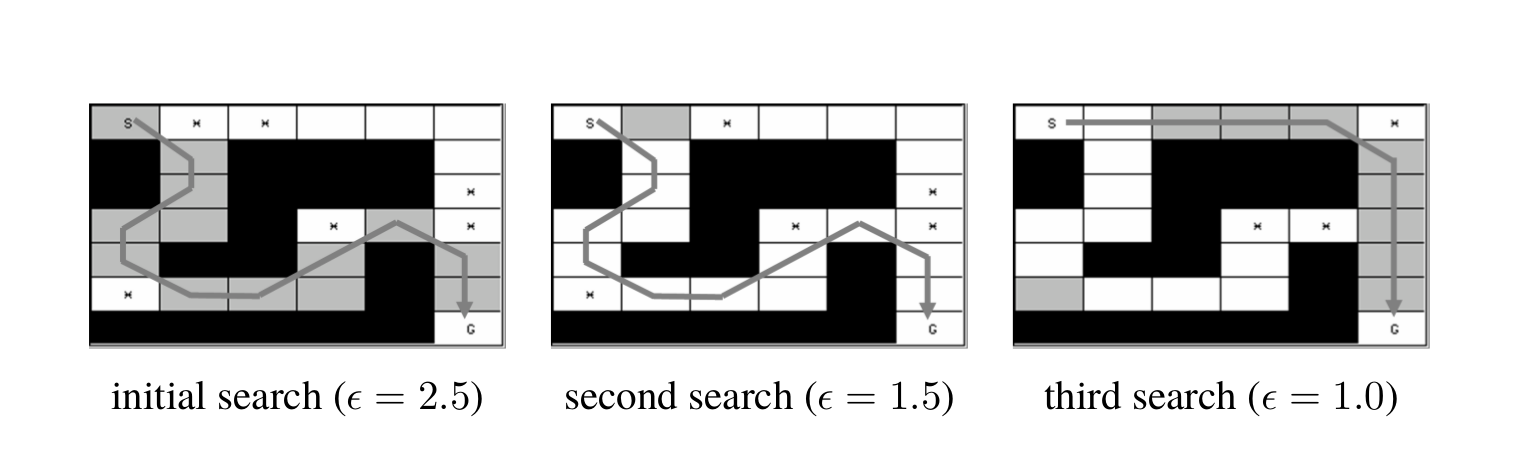
\includegraphics[width=.80\textwidth]{figuras/ara-3} 
\caption{Exemplo de aplicação da estratégia de diminuição do valor de $\epsilon$.}
\label{fig-ara-exemplo}
\end{figure}
\section{Algoritmo AD*}
\label{sec-dinamicos-ad}

O algoritmo AD* também proposto em \citeonline{likhachev2008anytime}, está descrito nas listagens \ref{lst-dinamicos-ad-set}, \ref{lst-dinamicos-ad-computepath}, \ref{lst-dinamicos-ad-key} e \ref{lst-dinamicos-ad-main}.

\begin{lstlisting}[mathescape, label=lst-dinamicos-ad-set, caption=Algoritmo AD* - função para determinar o conjunto ao qual vértice pertencerá, float=htpb]
procedure UpdateSetMembership(s)
	if ($v(s) \neq g(s)$)
		if (s $\notin$ CLOSED) insert/update s in OPEN with key(s);
		else if (s $\notin$ INCONS) insert s in INCONS;
	else
		if (s $\in$ OPEN) remove s from OPEN;
		else if (s $\in$ INCONS) remove s from INCONS;
\end{lstlisting}

\begin{lstlisting}[mathescape, label=lst-dinamicos-ad-computepath, caption=Algoritmo AD* - função de cálculo de caminho, float=htpb]
procedure ComputePath()
	while(key($s_{goal}$) > $min_{s \in OPEN(key(s))}$ OR v($s_{goal}$) < g($s_{goal}$)) 
		remove s with smallest key(s) from OPEN;
		if v(s) > g(s)
			v(s) = g(s); CLOSED = CLOSED $\cup$ {s};
			for each successor s' of s
				if s' was never visited by AD* before then
					v(s') = g(s') = $\infty$;bp(s') = null;
				if g(s') > g(s) + c(s, s')
					g(s') = g(s) + c(s, s');
					bp(s') = s;
					g(s') = g(bp(s')) + c(bp(s'),s'); UpdateSetMembership(s');
		else
			v(s) = $\infty$; UpdateSetMembership(s);
			for each successor s' of s
			if s' was never visited by AD* before then
				v(s') = g(s') = $\infty$;bp(s') = null;
			if bp(s') = s
				bp(s') = $argmin_{s'' \in pred(s')}$ v(s'') + c(s'',s');
				g(s') = v(bp(s')) + c(bp(s'),s'); UpdateSetMembership(s');
\end{lstlisting}

\begin{lstlisting}[mathescape, label=lst-dinamicos-ad-key, caption=Algoritmo AD* - função da chave ordenadora da fila de prioridades, float=htpb]
procedure key(s)
	if (v(s) $\geq$ g(s))
		return [g(s) + $\epsilon$ * h(s); g(s)];
	else
		return [v(s) + h(s); v(s)];
\end{lstlisting}

\begin{lstlisting}[mathescape, label=lst-dinamicos-ad-main, caption=Algoritmo AD* - função principal, float=htpb]
procedure Main()
	g($s_{goal}$) = v($s_{goal}$) = $\infty$; v($s_{start}$) = $\infty$;bp($s_{goal}$) = bp($s_{start}$) = null;
	g($s_{start}$) = 0; OPEN = CLOSED = INCONS = $\emptyset$; $\epsilon = \epsilon_{0}$;
	insert $s_{start}$ into OPEN with key($s_{start}$);
	forever
		ComputePath();
		publish current $\epsilon$-suboptimal solution;
		if $\epsilon = 1$
			wait changes in edge costs;
		for all directed edges (u,v) with changed edge costs
			update the edge cost c(u,v);
			if ( $v \neq s_{start}$ AND v was visited by AD* before)
				bp(v) = $argmin_{s'' \in pred(v)}$ v(s'') + c(s'',v);
				g(v) = v(bp(v)) + c(bp(v),v); UpdateSetMembership(v);
		if significant edge cost changes were observed
			increase $\epsilon$ or re-plan from scratch (i.e., re-excute Main function);
		else if $\epsilon > 1$
			decrease $\epsilon$;
		Move states from INCONS into OPEN
		Update the priorities for all s $\in$ OPEN according to key(s);
		CLOSED = $\emptyset$;
\end{lstlisting}

O algoritmo é muito semelhante em sua execução ao ARA*, já que o AD* é uma adaptação do mesmo \cite{moura2010estudo}. A função principal (listagem \ref{lst-dinamicos-ad-main}) começa iniciando os valores de g($s_{goal}$), v($s_{goal}$) e v($s_{start}$) como $\infty$, bp($s_{start}$) como nulo e g($s_{start}$) como 0. Em seguida o vértice $s_{start}$ é inserido na fila de prioridades de acordo com  a função de chave ordenadora descrita na listagem \ref{lst-dinamicos-ad-key}. Disso, é invocado a função de cálculo de caminho (listagem \ref{lst-dinamicos-ad-computepath}).

Essa função trabalha da seguinte forma: inicialmente se verifica se o valor da chave de $s_{goal}$ é maior do que a menor chave da fila de prioridades (condição semelhante ao do algoritmo ARA*, vide listagem \ref{lst-dinamicos-ara-computepath}) ou se o valor de v($s_{goal}$) é menor do que o valor de g( $s_{goal}$ ). Se caso for verdade, o processo iterativo é inciado. O vértice s, que corresponde ao vértice com menor chave na fila de prioridades é removido do conjunto OPEN, e é verificado se o valor de v(s) é maior do que o g(s) (ou seja, se o valor da distância calculada da busca anterior é maior do que o valor da busca atual, esse é o caso normal do algoritmo). Sendo verdade, o algoritmo segue a mesma forma de execução do ARA*, conforme descrito na seção \ref{sec-dinamicos-ara}. A diferença de tratamento ocorre quando a condição inicial não ocorre, e neste caso, o valor de v( s ) é atribuído como $\infty$, e para cada vértice s' adjacente de s é verificado se este já havia sido visitado pelo algoritmo. Se caso não havia sido visitado, os valores de v( s' ), g( s' ) são inciados como $\infty$ e bp( s') é inciado como nulo. Seguindo, é verificado se o bp( s' ) é igual o vértice s. Se caso sim, o bp( s' ) é atualizado com o vértice predecessor de s', s'', cuja a função v(s'') + c( s'', s') é a menor dentre todos os vértices predecessores de s'. Feito isso, o valor de g( s' ) é atualizado com esse novo valor. Em seguida a função de determinação para qual conjunto pertencerá s' é chamado (função "UpdateSetMembership").

A função de determinação ao qual conjunto pertencerá funciona de uma maneira muito simples. Caso os valores de v( s ) e g( s ) sejam diferentes, a função é igual ao que ocorre no processo de atribuição de conjunto do ARA* (vide listagem \ref{lst-dinamicos-ara-computepath}), a diferença ocorre quando esses valores são iguais (ou seja, não houve mudança de valores entre a busca atual e a anterior), o vértice é removido de OPEN caso esteja nele ou removido de INCONS caso pertença a este. Isso feito para que este vértice não precise ser calculada nesta busca ou na próxima (caso esteja em INCOS).

Voltando ao método principal (listagem \ref{lst-dinamicos-ad-main}), a função segue o mesmo padrão da ARA*, a única exceção se dá quando mudanças no grafo são detectadas (mudança dos pesos das arestas). Neste caso, para cada aresta (u,v) mudada, é atribuído ao valor bp( v ), o vértice s'', predecessor de v, cuja a função v( s'' ) + c( s'', v) seja mínima. Consequentemente, o valor de g( v ) é atualizado conforme esse valor e a função de atribuição de conjunto é invocada. 
% ==============================================================================
% TCC - Nome do Aluno
% Capítulo 5 - Testes Computacionais
% ==============================================================================
\chapter{Testes Computacionais}
\label{sec-testes}

\section{Algoritmo de Dijkstra}
\label{sec-dijkstra-experimentos}
Para a realização dos experimentos computacionais será rodado instâncias de grafos que representam malhas rodoviárias reais. Todas elas descritas nas tabelas \ref{tbl-dijkstra-instancias} e \ref{tbl-dijkstra-configuracao}, e disponíveis no sítio eletrônico \url{http://www.dis.uniroma1.it/challenge9/download.shtml} (acesso em 28 de janeiro de 2017).
\begin{table}[H]
\caption{Instâncias a serem rodadas pelo algoritmo de Dijkstra em suas três versões.}
\label{tbl-dijkstra-instancias}
\centering
\begin{adjustbox}{max width=\textwidth}
\begin{tabular}{|c|c|}
\hline 
\textbf{Nome Instância} & \textbf{Descrição} \\ 
\hline 
USA-road-d.NY.gr & Representa a malha viária do estado de Nova Iorque, Estados Unidos \\ 
\hline 
USA-road-d.BAY.gr & Representa a malha viária da bahia de São Francisco, Califórnia, Estados Unidos \\ 
\hline 
USA-road-d.COL.gr & Representa a malha viária do estado do Colorado, Estados Unidos \\ 
\hline 
USA-road-d.FLA.gr & Representa a malha viária do estado da Flórida, Estados Unidos \\ 
\hline 
\end{tabular}
\end{adjustbox}
\end{table}

\begin{table}[H]
\caption{Configuração dos grafos correspondestes as malhas viárias descritas na tabela \ref{tbl-dijkstra-instancias}.}
\label{tbl-dijkstra-configuracao}
\centering
\begin{adjustbox}{max width=\textwidth}
\begin{tabular}{|c|c|c|}
\hline 
\textbf{Nome Instância} & \textbf{Número de Vértices |V|} & \textbf{Número de Arestas |E|} \\ 
\hline 
USA-road-d.NY.gr
 & 264.346
 & 733.846
 \\ 
\hline 
USA-road-d.BAY.gr
 & 321.270
 & 800.172
 \\ 
\hline 
USA-road-d.COL.gr
 & 435.666
 & 1.057.066
 \\ 
\hline 
USA-road-d.FLA.gr
 & 1.070.376
 & 2.712.798
 \\ 
\hline 
\end{tabular}
\end{adjustbox} 
\end{table}

\subsection{Resultados obtidos}
\label{sec-dijkstra-experimentos-resultados}
Os resultados dos testes obtidos estão descritos a seguir.

\begin{figure}[H]
\centering
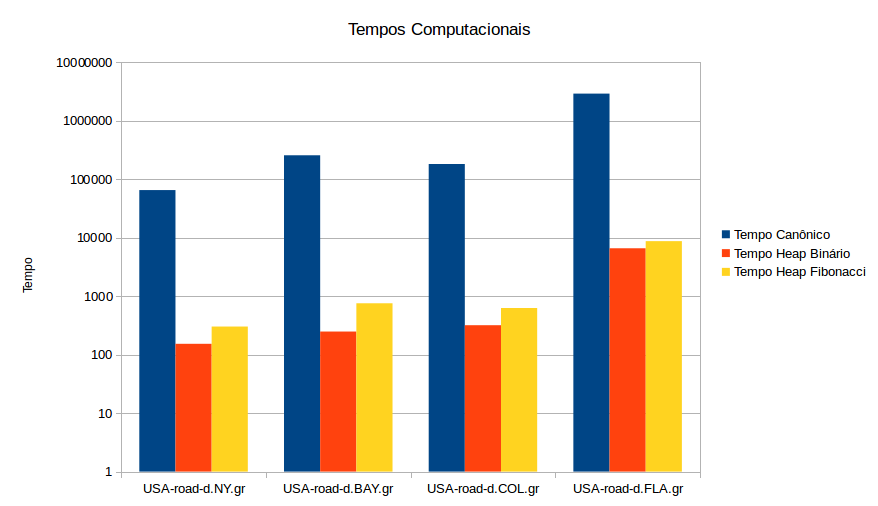
\includegraphics[width=.90\textwidth]{figuras/dijkstra-tempos} 
\caption{Tempos computacionais obtidos pelos Métodos de Dijkstra empregados (tempo em escala logarítmica).}
\label{fig-dijkstra-resultados-tempos}
\end{figure}

\begin{figure}[H]
\centering
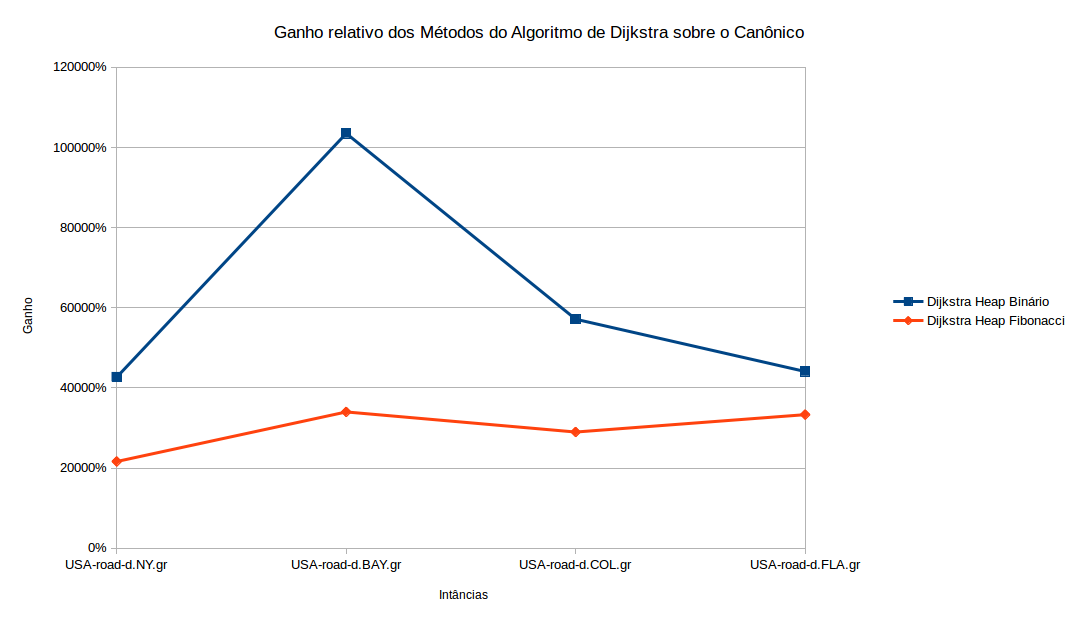
\includegraphics[width=.90\textwidth]{figuras/speed-up-dijkstra} 
\caption{Ganho relativo dos Métodos do Algoritmo de Dijkstra sobre o Canônico.}
\label{fig-dijkstra-resultados-speedup}
\end{figure}


\begin{table}[H]
\caption{Tempos Computacionais obtidos pelo algoritmo de Dijkstra em suas diferentes versões (tempo em milissegundos).}
\label{tbl-dijkstra-resultados-tempos}
\centering
\begin{adjustbox}{max width=\textwidth}
\begin{tabular}{|c|c|c|c|}
\hline
\textbf{Nome Instância} & \textbf{Tempo Canônico} & \textbf{Tempo Heap Binário} & \textbf{Tempo Heap Fibonacci} \\ \hline
USA-road-d.NY.gr        & 65287                   & 153                         & 302                           \\ \hline
USA-road-d.BAY.gr       & 256690                  & 248                         & 755                           \\ \hline
USA-road-d.COL.gr       & 181687                  & 318                         & 627                           \\ \hline
USA-road-d.FLA.gr       & 2909655                 & 6601                        & 8732                          \\ \hline
\end{tabular}
\end{adjustbox}
\end{table}


\begin{table}[H]
\caption{Ganho relativo sobre o Dijkstra Canônico.}
\label{tbl-dijkstra-resultados-speedup}
\centering
\begin{adjustbox}{max width=\textwidth}
\begin{tabular}{|c|c|c|}
\hline
\textbf{Nome Instância} & \textbf{Ganho Heap Binário} & \textbf{Ganho Heap Fibonacci} \\ \hline
USA-road-d.NY.gr        & 42.671\%                       & 21.618\%                         \\ \hline
USA-road-d.BAY.gr       & 103.504\%                      & 33.999\%                         \\ \hline
USA-road-d.COL.gr       & 57.134\%                       & 28.977\%                         \\ \hline
USA-road-d.FLA.gr       & 44.079\%                       & 33.322\%                         \\ \hline
\end{tabular}
\end{adjustbox}
\end{table}

\subsection{Análise dos resultados}
\label{sec-dijkstra-experimentos-analise}
Podemos observar que o Dijkstra Canônico elevou um tempo consideravelmente grande (a instância USA-road-d.FLA.gr por exemplo levou aproximadamente 48 minutos). Já o uso de estrutura de dados impactou consideravelmente no ganho do tempo sendo que o Heap Binário teve um ganho médio de 61.847\% com relação ao Dijkstra Canônico enquanto Dijkstra Heap de Fibonacci teve um ganho médio de 29.479\% (vide tabela \ref{tbl-dijkstra-resultados-speedup}).

Com relação ao resultado obtido pelos métodos do Heap Binário e Heap de Fibonacci, ele é de certo modo inesperado, já que conforme demonstrados nas subseções \ref{sec-dijkstra-versoes-heap} e \ref{sec-dijkstra-versoes-fibonacci}, o heap de Fibonacci possui tempo computacional, aplicado ao algoritmo de Dijkstra, de $O(|V|\lg |V| + |E|)$ enquanto o heap binário possui $O(|E| \lg |V|)$.  Como para todas as instâncias rodadas $|E| > |V|$ (vide tabela \ref{tbl-dijkstra-configuracao}), era de se esperar do ponto de vista teórico que a heap de Fibonacci apresentasse tempos mais rápidos do que o Heap Binário.

Porém, conforme também constatado por \citeonline{larkin2014back}, a aplicação prática das estruturas de dados nem sempre corresponde a esperada descrita na teoria. \citeonline{larkin2014back} mostram que estrutura de dados heaps baseadas em vetor são, na prática, mais eficientes do que a Heap de Fibonacci (vide referência para mais detalhes). É o que os testes realizados por este trabalho também constatam.

\subsection{Conclusões}
\label{sec-dijkstra-conclusoes}
Conforme demonstramos pelos experimentos descritos nesta seção, o algoritmo de Dijkstra que obteve o melhor resultado foi o Heap Binário, sendo mais rápido do que o próprio Heap de Fibonacci que teoricamente deveria ser mais rápido. O Dijkstra canônico obteve tempos que para aplicações como sistema de ponto global (em inglês, GPS) é indesejado, sendo sua implementação interessante apenas para fins de aprendizado e entendimento do algoritmo.

Em termos de implementação, sem dúvida o mais complicado para se implementar foi o Heap de Fibonacci devido a sua própria estrutura que contém uma lista circular duplamente encadeada (a lista de raízes), e pelas funções de restruturação da estrutura que possui muitas movimentações de nodos e tratamento de casos de desvio de condição.

Com isso, colocando em termos práticos, das formas de implementação apresentadas e testadas, a que melhor se sobressai é o Heap Binário que não só foi melhor no tempo dentre outros, como sua implementação é simples.

\section{Algoritmo A*}
\label{sec-aestrela-experimentos}

Para os experimentos computacionais serão utilizados as mesmas instâncias descritas em subseção \ref{sec-dijkstra-experimentos}. Serão comparados quatro versões de algoritmos: o algoritmo de Dijkstra descrito no capítulo \ref{sec-dijkstra}, o algoritmo de Dijkstra adaptado onde o algoritmo é parado assim que se é explorado o vértice objetivo, o algoritmo A* onde se utiliza a heurística admissível distância euclidiana e o algoritmo A* onde se utiliza a heurística não-admissível distância Manhattan, todas sumarizadas na tabela \ref{tbl-aestrela-instancias}.

\begin{table}[H]
\caption{Descrição das versões a serem testadas neste capítulo.}
\label{tbl-aestrela-instancias}
\centering
\begin{adjustbox}{max width=\textwidth}
\begin{tabular}{|c|c|}
\hline 
\textbf{Nome Instância} & \textbf{Descrição} \\ 
\hline 
Dijkstra & Versão de Dijsktra conforme descrito no capítulo \ref{sec-dijkstra} \\ 
\hline 
Dijkstra Adaptado & Versão de Dijkstra adaptado para parar quando o vértice destino é encontrado \\ 
\hline 
Algoritmo A* & Algoritmo A* utilizando a distância euclidiana \\ 
\hline 
Algoritmo A* Manhattan & Algoritmo A* utilizando a distância Manhattan \\ 
\hline 
\end{tabular} 
\end{adjustbox}
\end{table}

Será rodado dez vezes cada algoritmo para cada instância da subseção \ref{sec-dijkstra-experimentos} em que para cada rodada, será afixado o vértice origem como o sendo de valor de identificação "0" e terá como vértice destino um vértice escolhido aleatoriamente, sendo que não haverá repetição de vértices\footnote{Para o caso do algoritmo de Dijkstra especificado na primeira linha da tabela \ref{tbl-aestrela-instancias}, não será estabelecido um vértice destino já que o algoritmo calcula a melhor rota para todos os vértices do grafo.} (ou seja, supomos que o vértice de valor de identificação "180" tenha sido escolhido na primeira rodada. Esse vértice não será escolhido como destino nas demais 9 rodadas. Caso esse vértice seja "sorteado" na próxima iteração, um novo vértice será escolhido aleatoriamente). Nessas dez rodadas será verificado o tempo médio de execução, o número médio de vértices abertos por cada versão e para o algoritmo A* com a heurística Manhattan, será verificado a qualidade da solução.

Para todas as versões será utilizada a estrutura de dados Heap Binário (descrito na subseção \ref{sec-dijkstra-versoes-heap}) pois conforme mostrado no capítulo \ref{sec-dijkstra}, foi a estrutura que melhor se sobressaiu entre as outras em termos de tempo computacional.

\subsection{Resultados obtidos}
\label{sec-aestrela-instancias-resultados}

Os resultados dos testes computacionais descritos anteriormente podem ser vistos nas tabelas \ref{tbl-aestrela-resultados-tempo}, \ref{tbl-aestrela-resultados-qualidadesolucao} e \ref{tbl-aestrela-resultados-nva}.

\begin{table}[H]
\caption{Tempo médio obtido pelos métodos descritos na tabela \ref{tbl-aestrela-instancias} (tempo em milissegundos).}
\label{tbl-aestrela-resultados-tempo}
\centering
\begin{adjustbox}{max width=\textwidth}
\begin{tabular}{|c|c|c|c|c|}
\hline
\textbf{Nome Instância} & \textbf{Dijkstra} & \textbf{Dijkstra Adaptado} & \textbf{Algoritmo A*} & \textbf{Algoritmo A* Manhattan} \\ \hline
USA-road-d.NY.gr        & 236                           & 109                                    & 29                      & 14                                \\ \hline
USA-road-d.BAY.gr       & 321                           & 187                                    & 54                      & 23                                \\ \hline
USA-road-d.COL.gr       & 494                           & 229                                    & 117                     & 27                                \\ \hline
USA-road-d.FLA.gr       & 2858                          & 1026                                   & 886                     & 101                               \\ \hline
\end{tabular} 
\end{adjustbox}
\end{table}

\begin{table}[H]
\caption{Diferença média de solução obtida pelo A* Manhattan com relação a solução ótima.}
\label{tbl-aestrela-resultados-qualidadesolucao}
\centering
\begin{adjustbox}{max width=\textwidth}
\begin{tabular}{|c|c|}
\hline
\textbf{Nome Instância} & \textbf{Qualidade Solução} \\ \hline
USA-road-d.NY.gr        & 5\%                        \\ \hline
USA-road-d.BAY.gr       & 4\%                        \\ \hline
USA-road-d.COL.gr       & 3\%                        \\ \hline
USA-road-d.FLA.gr       & 3\%                        \\ \hline
\end{tabular} 
\end{adjustbox}
\end{table}

\begin{table}[H]
\caption{Número de Vértices Abertos (NVA) médio por cada método.}
\label{tbl-aestrela-resultados-nva}
\centering
\begin{adjustbox}{max width=\textwidth}
\begin{tabular}{|c|c|c|c|}
\hline
\textbf{Nome Instância} & \textbf{NVA Dijkstra Adptado} & \textbf{NVA A*} & \textbf{NVA A* Manhattan} \\ \hline
USA-road-d.NY.gr        & 140501                        & 31995           & 9079                      \\ \hline
USA-road-d.BAY.gr       & 225754                        & 53206           & 17044                     \\ \hline
USA-road-d.COL.gr       & 242674                        & 108343          & 21577                     \\ \hline
USA-road-d.FLA.gr       & 580010                        & 349201          & 79077                     \\ \hline
\end{tabular} 
\end{adjustbox}
\end{table}

\subsection{Análise dos resultados}
\label{sec-aestrela-resultados-analise}
Como apontado pelos testes realizados, o algoritmo A* teve um desempenho computacional melhor do que o algoritmo Dijkstra, inclusive sobre o Dijkstra Adaptado (descrito anteriormente). Podemos ver que esse resultado está diretamente ligado ao número de vértices abertos por cada algoritmo (tabela \ref{tbl-aestrela-resultados-nva}). Aqueles que abriram mais vértices, obtiveram um tempo computacional maior. Isso já esperado, já que o algoritmo teve que processar mais etapas até que sua condição de parada fosse encontrada.

Dos quatro métodos testados, o que obteve menor tempo computacional foi o algoritmo A* aplicando a heurística não-admissível Distância Manhattan. Isso se deve ao fato de o cálculo da distância (que é realizado em tempo de execução) ser mais simples do que o empregado pela distância euclidiana (que envolve radiação e exponenciação). Porém esse resultado possui um "preço a ser pago" que é, conforme descrito na subseção \ref{sec-aestrela-algoritmo-heuristica}, a não garantia do menor caminho entre os vértices pesquisados. Mas, conforme demonstra a tabela \ref{tbl-aestrela-resultados-qualidadesolucao}, a diferença média entre as soluções encontradas e suas respectivas soluções ótimas giram em torno de 4\%, o que pode ser considerado como um bom resultado.

\subsection{Conclusões}
\label{sec-aestrela-conclusao}
O algoritmo A* demonstra ser um ótimo algoritmo para o cálculo de menor caminho entre dois vértices (origem e destino), superando em tempo computacional o algoritmo de Dijsktra (mas que retorna a menor rota para todos os demais vértices), sendo mais indicado para esse tipo de cálculo. Sua implementação é simples e é praticamente uma adaptação do algoritmo de Dijsktra.

Com relação as heurísticas, para a garantia do melhor caminho como o algoritmo de Dijkstra o faz, é obrigatório o uso de uma heurística admissível, mesmo que isso tenha um impacto negativo no tempo com relação ao uso de outras heurísticas (as não-admissíveis). Porém, conforme mostrado na subseção ref{sec-aestrela-instancias-resultados}, a diferença entre as soluções ótimas e obtidos pelo método Manhattan giraram em torno de 4\%, o que é um bom resultado para quem deseja menor tempo computacional e não possui a obrigatoriedade do menor caminho.

\section{Algoritmos Dinâmicos}
\label{sec-experimentos-dinamicos}
Para o capítulo de algoritmo dinâmicos serão rodados dois tipos testes, um para cada algoritmo. Serão utilizadas as mesmas instâncias descritas na seção \ref{sec-dijkstra-experimentos}.

\subsection{ARA*}
\label{sec-experimentos-dinamicos-ara}

Para os testes com o algoritmo ARA*, será comparado o desempenho da utilização da heurística inflada com relação ao desempenho do algoritmo de Dijkstra. Será afixado um conjunto arbitrário de $\epsilon$ e será medido quanto tempo o algoritmo ARA* acha uma solução (mesmo não sendo a ótima) para aquele determinado $\epsilon$ e comparar com o tempo que o algoritmo A* acha uma solução ótima, além do número médio de vértices abertos por cada algoritmo. Será utilizada a mesma forma de bateria de testes descritas na seção \ref{sec-aestrela-experimentos} em que serão escolhidos 10 vértices diferentes aleatórios como vértice destino e 0 como vértice origem e depois disso, tirado a média dos tempo total gasto para achar a rota.

\subsubsection{Resultados obtidos}
\label{sec-experimentos-dinamicos-ara-resultados}

Os resultados dos experimentos estão descritos a seguir na tabela \ref{tbl-experimentos-dinamicos-ara}. O tempo é descrito em nanosegundos (ns). Observe também que o valor do tempo médio do algoritmo A* não varia dentro da mesma instância. Isso é devido a ser utilizado o resultado único para cada estância, já que o valor de $\epsilon$ não é utilizado pelo A*.

\begin{table}[H]
\caption{Resultado testes ARA*.}
\label{tbl-experimentos-dinamicos-ara}
\centering
\begin{adjustbox}{max width=\textwidth}
\begin{tabular}{|c|c|c|c|c|c|c|}
\hline
\textbf{Nome Instância}            & \multicolumn{1}{l|}{\textbf{Epsisolon}} & \multicolumn{1}{l|}{\textbf{NVA A*}} & \multicolumn{1}{l|}{\textbf{Tempo médio A*}} & \multicolumn{1}{l|}{\textbf{NVA ARA*}} & \multicolumn{1}{l|}{\textbf{Tempo médio ARA*}} & \multicolumn{1}{l|}{\textbf{Ganho de tempo com realção ao A*}} \\ \hline
\multirow{7}{*}{USA-road-d.NY.gr}  & 4.0                                     & 29394                                & 26900000                                     & 252                                    & 980000                                         & 2.700\%                                                        \\ \cline{2-7} 
                                   & 3.5                                     & 29394                                & 26900000                                     & 257                                    & 320000                                         & 8.400\%                                                        \\ \cline{2-7} 
                                   & 3.0                                     & 29394                                & 26900000                                     & 265                                    & 820000                                         & 3.200\%                                                        \\ \cline{2-7} 
                                   & 2.5                                     & 29394                                & 26900000                                     & 281                                    & 840000                                         & 3.200\%                                                        \\ \cline{2-7} 
                                   & 2.0                                     & 29394                                & 26900000                                     & 296                                    & 560000                                         & 4.800\%                                                        \\ \cline{2-7} 
                                   & 1.5                                     & 29394                                & 26900000                                     & 360                                    & 940000                                         & 2.800\%                                                        \\ \cline{2-7} 
                                   & 1.0                                     & 29394                                & 26900000                                     & 4825                                   & 3140000                                        & 800\%                                                          \\ \hline
\multirow{7}{*}{USA-road-d.BAY.gr} & 4.0                                     & 43896                                & 45980000                                     & 239                                    & 1180000                                        & 3.800\%                                                        \\ \cline{2-7} 
                                   & 3.5                                     & 43896                                & 45980000                                     & 236                                    & 800000                                         & 5.700\%                                                        \\ \cline{2-7} 
                                   & 3.0                                     & 43896                                & 45980000                                     & 224                                    & 800000                                         & 5.700\%                                                        \\ \cline{2-7} 
                                   & 2.5                                     & 43896                                & 45980000                                     & 233                                    & 620000                                         & 7.400\%                                                        \\ \cline{2-7} 
                                   & 2.0                                     & 43896                                & 45980000                                     & 252                                    & 1040000                                        & 4.400\%                                                        \\ \cline{2-7} 
                                   & 1.5                                     & 43896                                & 45980000                                     & 299                                    & 740000                                         & 6.200\%                                                        \\ \cline{2-7} 
                                   & 1.0                                     & 43896                                & 45980000                                     & 10867                                  & 7920000                                        & 500\%                                                          \\ \hline
\multirow{7}{*}{USA-road-d.COL.gr} & 4.0                                     & 69991                                & 68140000                                     & 99                                     & 580000                                         & 11.700\%                                                       \\ \cline{2-7} 
                                   & 3.5                                     & 69991                                & 68140000                                     & 93                                     & 860000                                         & 7.900\%                                                        \\ \cline{2-7} 
                                   & 3.0                                     & 69991                                & 68140000                                     & 92                                     & 780000                                         & 8.700\%                                                        \\ \cline{2-7} 
                                   & 2.5                                     & 69991                                & 68140000                                     & 92                                     & 720000                                         & 9.400\%                                                        \\ \cline{2-7} 
                                   & 2.0                                     & 69991                                & 68140000                                     & 90                                     & 500000                                         & 13.600\%                                                       \\ \cline{2-7} 
                                   & 1.5                                     & 69991                                & 68140000                                     & 172                                    & 580000                                         & 11.700\%                                                       \\ \cline{2-7} 
                                   & 1.0                                     & 69991                                & 68140000                                     & 2080                                   & 1720000                                        & 3.900\%                                                        \\ \hline
\multirow{7}{*}{USA-road-d.FLA.gr} & 4.0                                     & 255312                               & 711120000                                    & 808                                    & 3500000                                        & 20.300\%                                                       \\ \cline{2-7} 
                                   & 3.5                                     & 255312                               & 711120000                                    & 840                                    & 2820000                                        & 25.200\%                                                       \\ \cline{2-7} 
                                   & 3.0                                     & 255312                               & 711120000                                    & 913                                    & 2460000                                        & 28.900\%                                                       \\ \cline{2-7} 
                                   & 2.5                                     & 255312                               & 711120000                                    & 596                                    & 2220000                                        & 32.000\%                                                       \\ \cline{2-7} 
                                   & 2.0                                     & 255312                               & 711120000                                    & 524                                    & 1940000                                        & 36.600\%                                                       \\ \cline{2-7} 
                                   & 1.5                                     & 255312                               & 711120000                                    & 687                                    & 2060000                                        & 34.500\%                                                       \\ \cline{2-7} 
                                   & 1.0                                     & 255312                               & 711120000                                    & 18909                                  & 14360000                                       & 4.900\%                                                        \\ \hline
\end{tabular}
\end{adjustbox}
\end{table}

\subsubsection{Análise dos resultados}
\label{sec-experimentos-dinamicos-ara-analise}




% ==============================================================================
% TCC - Nome do Aluno
% Capítulo 5 - Testes Computacionais
% ==============================================================================
\chapter{Considerações Finais e Trabalhos Futuros}
\label{sec-conclusao}

Neste trabalho foram realizados estudos de algoritmos de caminho mínimo para grafos estáticos e dinâmicos, abordando seus funcionamentos, suas estratégias e o impacto que o uso de determinadas estruturas de dados ocasionam. Por meio dos testes computacionais realizados foi possível constatar a eficácia desses algoritmos e analisar em quais situações melhor se aplicam.

Foram estudados os algoritmos de Dijkstra, busca A*, \textit{Anytime Repairing} A* (ARA*) e o \textit{Anytime Dynamic} A* (AD*) sobre instâncias que representam malhas rodoviárias reais, sendo o número de vértices e arestas desses grafos, da ordem de grandeza de 100.000 a 1.000.000, possibilitando assim verificar o desempenho desses algoritmos em uma situação real e verificando também o desempenho para diferentes tamanhos de grafos.

Este trabalho constatou que a escolha de uma determinada estrutura de dados impacta fortemente no desempenho do algoritmo e que certas estrutura de dados propostas, como é o caso da heap de Fibonacci, apesar de teoricamente possuírem análise computacional melhor do que outras estruturas de dados como a heap binária, na prática, nem sempre é essa situação que ocorre, tendo fatores práticos computacionais que prejudicam o desempenho. Foi possível constatar também que o algoritmo A*, em geral, tem um desempenho melhor do que o algoritmo de Dijkstra devido ao uso da estratégia de heurística e de ser objetivo ao se determinar um vértice destino a ser buscado um caminho (em detrimento do Dijkstra que busca a solução calculando a melhor rota para todos os caminhos, sendo seu uso mais recomendado quando a aplicação exige a melhor rota para mais de um vértice). Foi verificado também que o uso de heurísticas não-admissíveis, apesar de se perder a garantia do resultado ótimo, obtêm bons ganhos de tempos computacionais a um preço baixo de deterioramento de qualidade de solução que gira em torno de 4\%. Para os algoritmos dinâmicos, constatou-se que o algoritmo AD* se adéqua muito bem a esse tipo de grafo, tendo que ao se detectar mudança no peso de suas arestas, o algoritmo consegue calcular uma nova rota sem ter que recalcular todos os vértices que antes seriam necessários para achar uma nova rota, já que se baseia no uso de vértices já calculados anteriormente. Já o algoritmo ARA* se mostra muito eficiente para o cálculo rápido de soluções, que não são garantidamente ótimas, mas que a medida que o tempo for passando, essa solução tem a possibilidade de ser melhorada a um custo menor do que se fosse recalculada utilizando todos os vértices necessários.

Para trabalhos futuros sugerimos realizar testes para comparar o desempenho dos algoritmos AD* e ARA* com o D* e o D* Lite, que são algoritmos dinâmicos propostos em \citeonline{stentz1994optimal} e \citeonline{koenig2002d} respectivamente, verificando também em quais situações cada um melhor se aplica. Além disso, vale também um estudo do uso de outras heurísticas além das que foram aplicadas, tanto para o algoritmo A* quanto para o ARA* e o AD*, incluindo também, nestes dois últimos casos, o uso de heurísticas não-admissíveis. Para o algoritmo de Dijkstra sugere a realização de testes com outras estruturas de dados propostas que não foram testadas por este trabalho.



%%% Páginas finais do documento: bibliografia e anexos. %%%

% Finaliza a parte no bookmark do PDF para que se inicie o bookmark na raiz e adiciona espaço de parte no sumário.
\phantompart

% Marca o início dos elementos pós-textuais.
\postextual

% Referências bibliográficas
\bibliography{bibliografia}


% Apêndices.



% Índice remissivo.
\phantompart
\printindex

% Fim do documento.
\end{document}
